\documentclass[12pt,twoside]{report}

% some definitions for the title page
\newcommand{\reporttitle}{The Emotion Engine}
\newcommand{\reportauthor}{Kaede Sugano}
\newcommand{\supervisor}{William Knottenbelt}
\newcommand{\reporttype}{Undergraduate Individual Project}
\newcommand{\degreetype}{MEng} 

% load some definitions and default packages
\input{includes}

% load some macros
\input{notation}

% load title page
\begin{document}
\input{titlepage}


% page numbering etc.
\pagenumbering{roman}
\clearpage{\pagestyle{empty}\cleardoublepage}
\setcounter{page}{1}
\pagestyle{fancy}

%%%%%%%%%%%%%%%%%%%%%%%%%%%%%%%%%%%%
\begin{abstract}
Verbalisation is a lossy compression of emotional experience. Natural language forces continuous affective states into discrete lexical categories, collapsing the subtle blends and gradations that precede and motivate linguistic output. This work investigates whether large language models encode a richer pre-verbal emotion representation in their internal activations, separable from surface lexical content, and whether that representation can be geometrically decomposed and causally manipulated.\par

We propose a two-level decomposition of affective structure in the residual stream of Llama-3.1-8B-Instruct. At the first level, CAA vectors computed for eight Plutchik emotions are dominated by a shared emotionalisation direction $\mathbf{g}$. Projecting out $\mathbf{g}$ yields emotion-specific residual prototypes $\hat{\mathbf{r}}_e$ that recover Plutchik's circular geometry. At the second level, within-emotion residuals are decomposed via pooled PCA into affective texture axes $\mathbf{m}_k$, which modulate arousal, temporal orientation, and social engagement independently of emotion identity. Two independent extraction methods converge at cosine similarities of $\geq 0.931$, ruling out methodological artefact. The full steering formula is $\Delta_e = \alpha_R \hat{\mathbf{r}}_e + \sum_k \gamma_k \mathbf{m}_k$.\par

A human evaluation ($N = 18$) confirms both levels are perceptually distinguishable: $84.4\%$ of forced-choice judgements correctly identified the predicted arousal pole of $\mathbf{m}_1$ ($p < 0.001$), emotion categories were preserved in $91.7\%$ of steered outputs, and prototype steering raised Likert ratings by $+1.97$ points on average. Together, these findings show that affective generation decomposes into geometrically meaningful, causally active components that are perceptible to human readers.\par
\end{abstract}

\cleardoublepage
%%%%%%%%%%%%%%%%%%%%%%%%%%%%%%%%%%%%
\section*{Acknowledgments}

I would like to express my sincere gratitude to Professor William Knottenbelt, who has supported me since my Year 3 group project and kindly offered to support me in any way when I first proposed my own project idea. I am also grateful to Professor Ben Glocker, my second marker, for his valuable and constructive feedback after the interim report, which helped me reflect on and improve the direction of this work.\par

I would also like to thank all of my friends who took part in the human evaluation. In particular, thanks to Ryota, Vlad, Ray and Yurika for reading my report, encouraging me by telling me that the idea was exciting, and patiently helping me correct my English grammar many times!\par

\clearpage{\pagestyle{empty}\cleardoublepage}

%%%%%%%%%%%%%%%%%%%%%%%%%%%%%%%%%%%%
%--- table of contents
\fancyhead[RE,LO]{\sffamily {Table of Contents}}
\tableofcontents


\clearpage{\pagestyle{empty}\cleardoublepage}
\pagenumbering{arabic}
\setcounter{page}{1}
\fancyhead[RO]{\small\parbox[t]{0.75\textwidth}{\raggedleft\textsl{\rightmark}}}
\fancyhead[LE]{\small\parbox[t]{0.75\textwidth}{\raggedright\textsl{\leftmark}}}
\fancyhead[LO,RE]{}

%%%%%%%%%%%%%%%%%%%%%%%%%%%%%%%%%%%%
\chapter{Introduction}
\label{chap:introduction}

\section{Words draw boundary lines across the ocean of ``concepts''}
When I was still in elementary school, my favourite biography in the library was Helen Keller's. Stricken by illness as a child, she lost both sight and hearing and bore the ``triple hardship'' of being blind, deaf, and mute, yet devoted herself to the advancement of education and welfare for the disadvantaged.

But Helen Keller's story is not merely a tale of ``overcoming adversity.'' What is etched most vividly in my memory is the moment when she first understood the word ``water.'' At first, Helen insisted that ``cup'' and ``the water in it'' were the same thing. However, the instant when Anne Sullivan signed ``W-A-T-E-R'' into her hand while letting the cold water from a pump run across Helen's palm, her world changed. When she could separate the object that flows from the container, the continuum of chaos was reshaped into an ordered world with partitions.

This scene exemplifies the essence of language. We do not grasp the external world directly as ``things-in-themselves.'' The information flowing into our senses is, in truth, a continuum; language draws borders there and carves out units of meaning. Even the boundary between river and sea is not sharply inscribed by nature itself; it is defined for human convenience and by culture~-- ``this far is river,'' ``from here is sea.'' Words do not merely copy lines already inscribed upon the world; they are the very act of drawing those lines as needed. In other words, language is not just a label: it is the activity by which we impose boundaries within our cognition and shape the world we see. To learn words is not merely to expand vocabulary; it is to gain a way of partitioning the ocean of concepts and choosing how to look at the world. In that sense, we are, day by day, sketching new boundaries.

\section{Verbalisation is a lossy compression}
Verbalisation is an act of forcing the complex and continuous sensation into discretised vocabulary and grammar. When we perform \textbf{verbalisation}, there lurks a commonly overlooked risk; it is intrinsically \textbf{lossy}. The moment we verbalise, the fine nuances contained within raw feeling are abstracted into the fences of cognition that humanity has drawn at the level of words. Even if we choose the same term, the warmth that term carries depends on each person's embodied history, and it is eventually averaged out. The relief or pride we felt when we opened our old school yearbook for the first time in a decade, once put into text, may be flattened into a bland ``how nostalgic.'' Moreover, lexicons and meanings for emotions differ greatly across languages and cultures\cite{jackson2019emotion}; terms like ``anger'' or ``joy'' do not necessarily point to the same nuances around the world. And yet humanity cannot let go of language. Even if it is a lossy compression, language remains the only standardised interface that connects the human heart to society.


\section{Objectives}
The goal of this project is not to deny language but to design a parallel circuit that supplements the components lost in the compression of verbalisation, i.e.\ a circuit for restoring what words leave behind. What if we could scoop up the human central cognition directly, without passing through the rendering pipeline of language, and translate it into other forms of expression? Could we transfer the lingering sensation that arises when reading a letter from your significant other into poetry or essays? Or could we improve novel translations by capturing emotions lost through differences in lexical definitions between languages? Here lies an uncharted gap in our understanding of human cognition. 

This project aims to emulate a kind of human synaesthesia. In other words, we aim to map emotions across modalities. We will develop the foundational technology to extract, manipulate, and re-synthesise a \textbf{pre-verbal, intermediate representation of emotion}, and explore possible ways to steer the model output using those representations of emotion.

The final product of this project is a computational system capable of extracting, manipulating, and presenting the emotions contained in input text without having to go through the compression of verbalisation.
The system focuses not on what the text superficially tells, but on the emotional state that existed immediately before the text was produced, and treats it as a continuous vector representation.

When a user enters any text, the system analyses the emotional nuances contained in that text and visualises them as a low-dimensional continuous vector. These emotion vectors are not discrete labels such as ``joy'' and ``sadness,'' but are expressed as multiple overlapping emotional directions, thus preserving subtle mixed emotions and fluctuations that cannot be captured by language.

Users can intuitively manipulate this emotion code space. For example, by strengthening only a specific emotional direction and weakening another direction for the simultaneous presence of \texttt{relief} and \texttt{loneliness} in a certain sentence, it is possible to sensitively edit the emotional state that one really wanted to convey. It is important to note that this operation is not performed at the linguistic level, such as vocabulary selection or stylistic adjustment, but rather on the emotional expression itself before the language is generated.

The edited emotion code is again transformed into a linguistic expression. The text generated here is not simply a paraphrased sentence, but is the result of a re-expression that retains or intentionally transforms the emotion contained in the original sentence.

In this process, the user does not need to put their emotions into explicit words. The verbal averaging and simplification that is usually considered inevitable between emotion recognition and generation is bypassed, and the raw emotion felt by the user can be transferred to another form of expression in a more controllable manner.

This end product is neither a system for classifying and diagnosing emotions nor a tool for automatically generating emotional sentences. Rather, it is an interface that temporarily holds the emotions that people had before they put them into words as manipulatable intermediate expressions, from which new linguistic expressions can be launched. The ultimate value of this project lies in the fact that it makes it possible to return to the boundaries drawn by language and choose words again.


%%%%%%%%%%%%%%%%%%%%%%%%%%%%%%%%%%%%
\chapter{Background}

\section{Emotion Representation in LLMs}

\subsection{Discrete Emotion Labels and Their Limitations}

Early work treated emotion as a small set of discrete categories. The most influential taxonomy is Ekman's seven basic emotions: anger, contempt, disgust, enjoyment, fear, sadness, and surprise~\cite{ekman1999basic}. 

\begin{figure}[H]
    \centering
    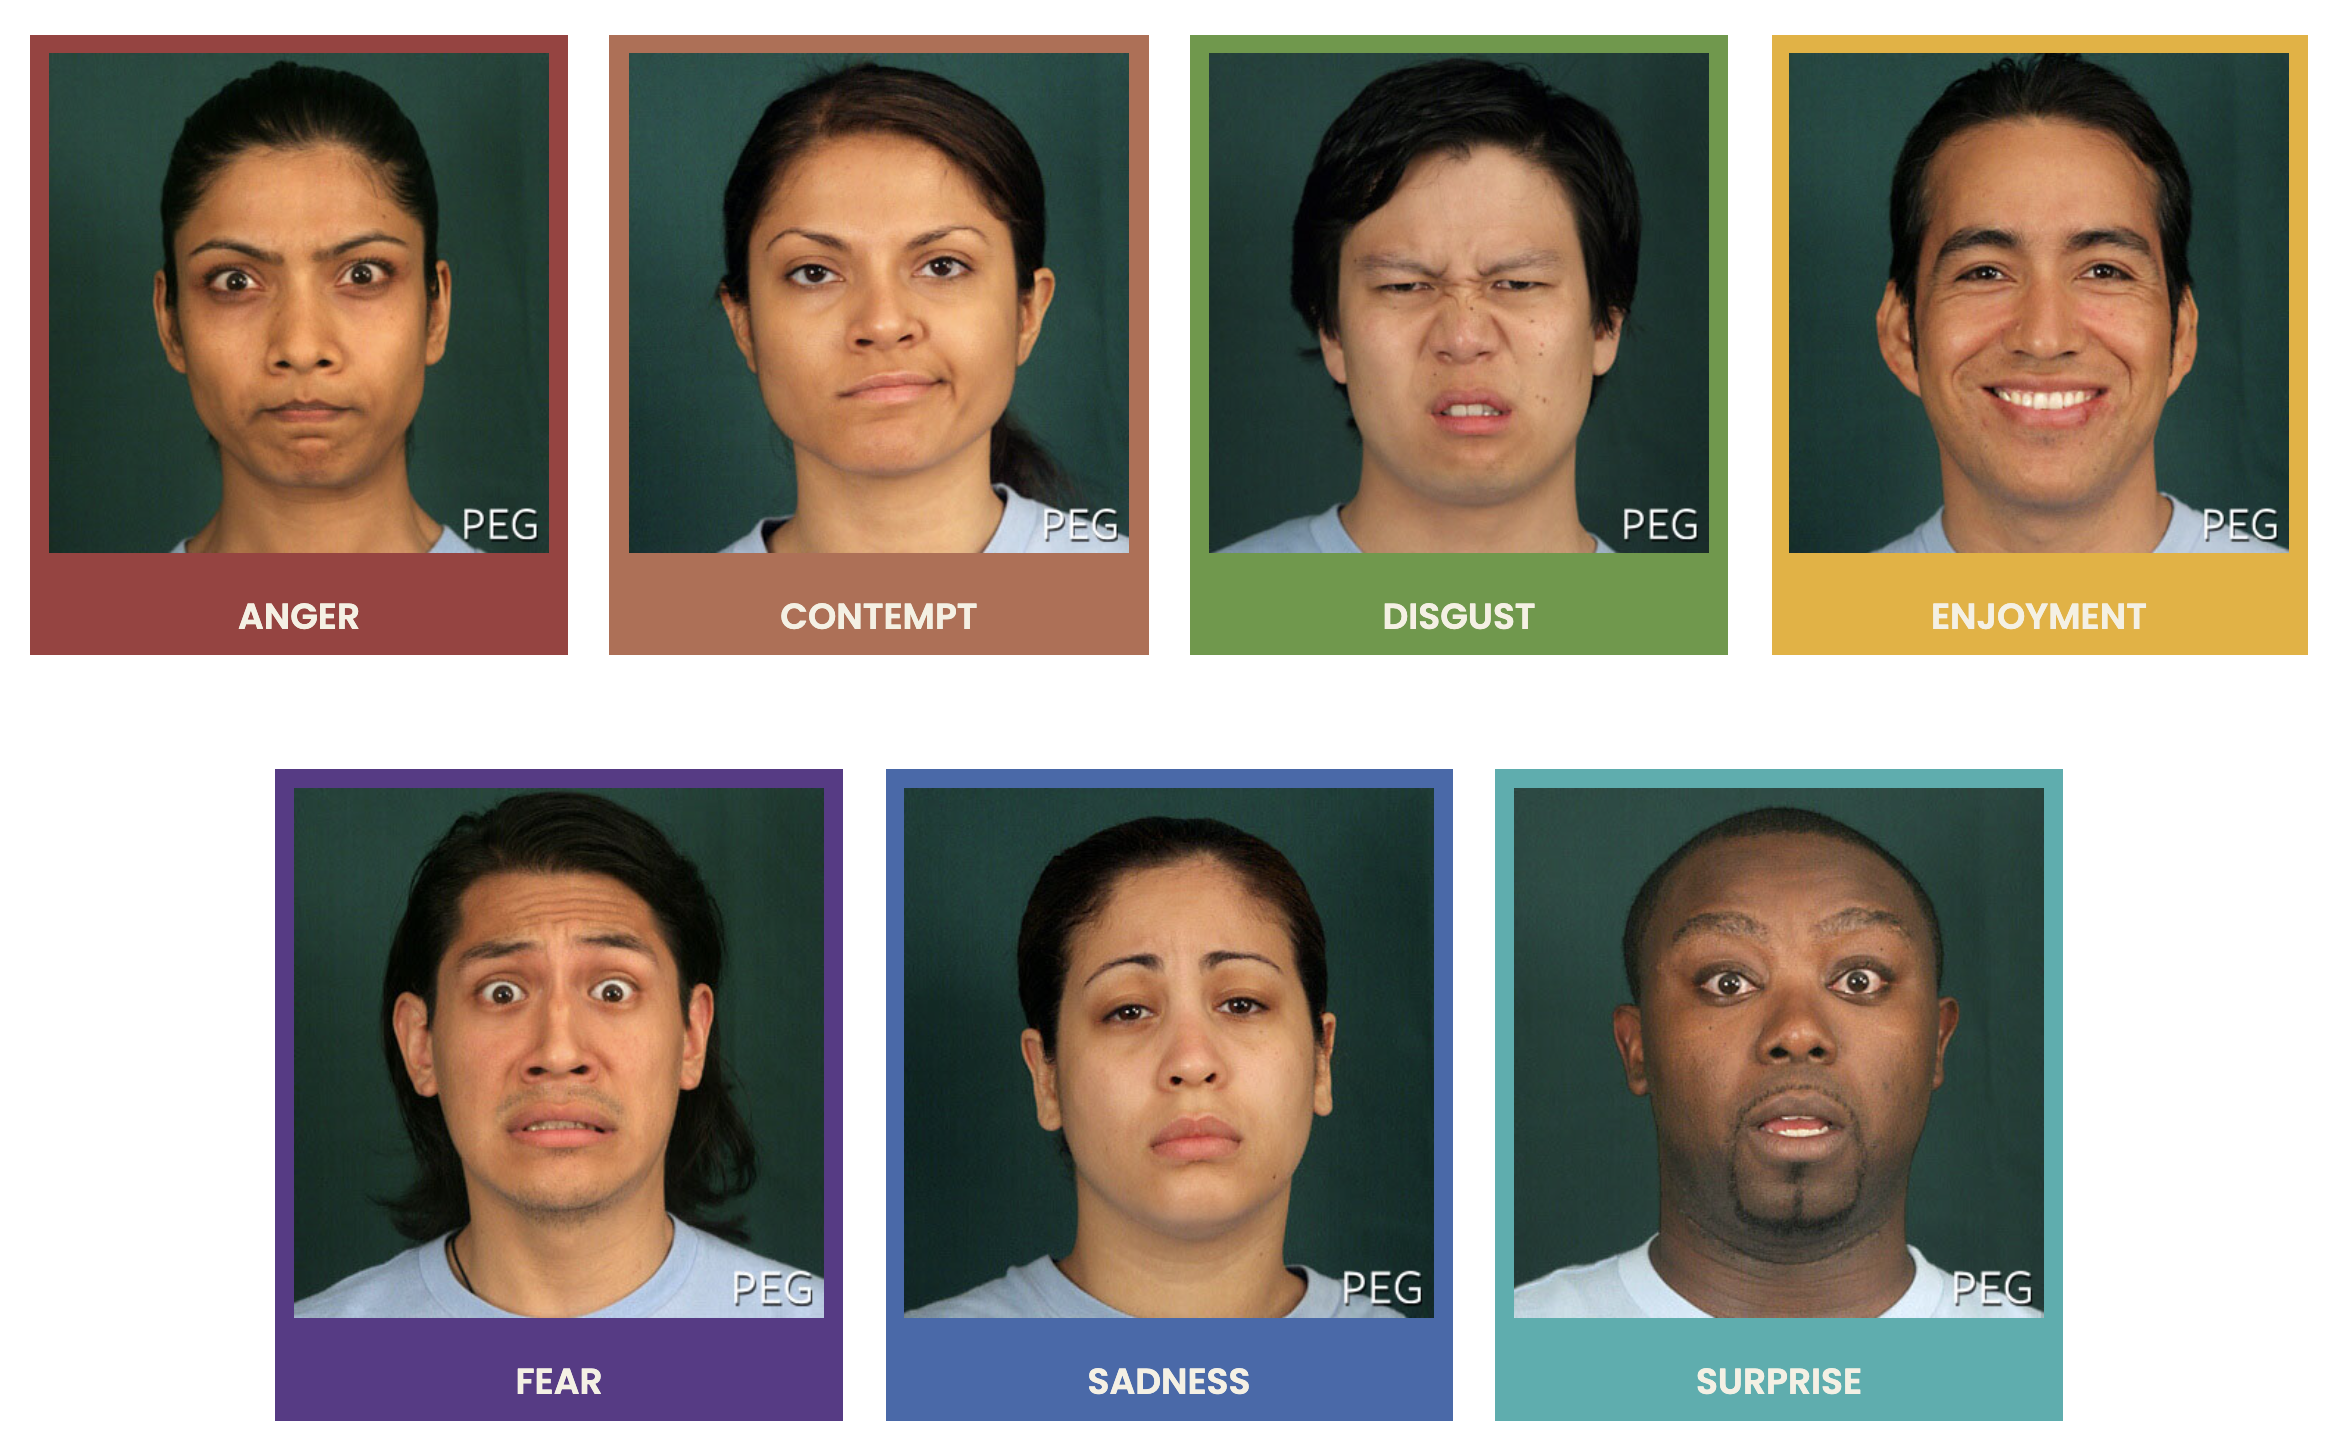
\includegraphics[width=0.5\linewidth]{figures/paul_ekman.png}
    \caption{Paul Ekman's seven basic emotions~\cite{paul_ekman_web}}
    \label{fig:paul_ekman}
\end{figure}

This assumes that emotions are biologically universal and psychologically irreducible. This framework enabled early supervised emotion classification systems by providing a clear labeling scheme and facilitated the construction of benchmark datasets. However, the categorical assumption introduces strong inductive bias; emotions are treated as mutually exclusive and qualitatively distinct.

Subsequent datasets attempted to increase expressive granularity. GoEmotions~\cite{demszky2020goemotionsdatasetfinegrainedemotions}, for example, expanded the label space to 27 emotion categories and allowed multi-label annotation. 

\begin{figure}[H]
    \centering
    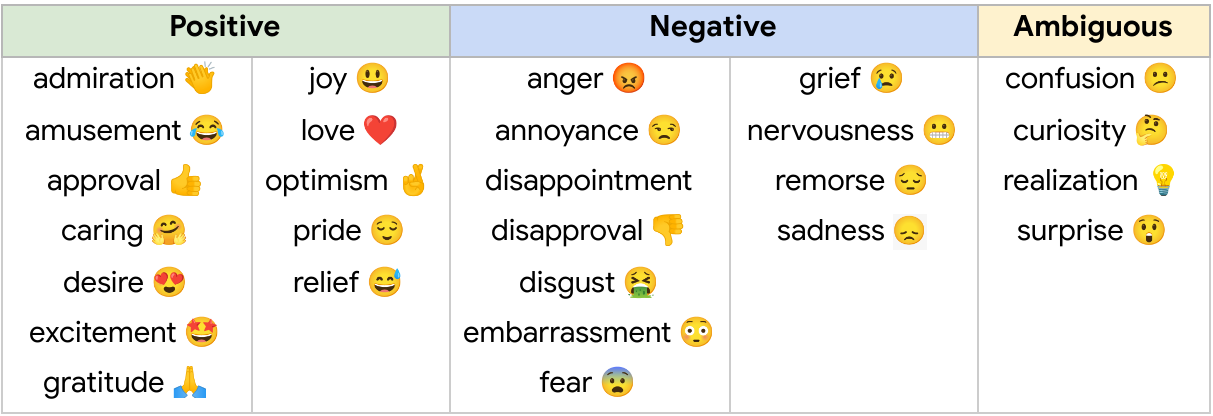
\includegraphics[width=0.8\linewidth]{figures/goemotions.png}
    \caption{GoEmotions taxonomy: 28 emotion categories including ``neutral''.~\cite{goemo}}
    \label{fig:goemotions}
\end{figure}

This enabled us to capture cases where multiple emotions occur in a single utterance. It is reported that emotions cluster by sentiment polarity and intensity, and that many categories exhibit high inter-label correlation. Nevertheless, despite its increased resolution, the dataset still relies on one-hot / sparse multi-hot encodings. Such encodings collapse emotional intensity and compositional structure into discrete indices, preventing the representation of graded transitions. For example, the difference between mild and intense anger cannot be represented, and the blend of emotions, such as bittersweet emotion, is also difficult.

Essentially, discrete labels force the learning problem into a classification regime that cannot capture continuity, geometry, or arithmetic structure. For example, two samples labeled \texttt{joy} may be emotionally distant, while \texttt{joy} and \texttt{contentment} may be emotionally close; yet this structure is invisible to the model itself. These limitations motivate a shift away from purely categorical representations toward continuous emotion spaces.

This problem of the discretised emotion labels is also raised  by Wang and Zong (2021)~\cite{wang-zong-2021-distributed}. They explicitly formalise this by arguing that one-hot emotion labels ignore latent relationships between emotion categories. They observe that emotion calsses are not orthogonal in human perception, but rather exhibit similarity in a gradation manner. More broadly, discrete labeling schemes prioritises  the annotation convenience over the representational adequacy. While it simplify supervision and evaluation, they impose artificial bounadies that obscure the underlying structure of emotions. This mismatch becomes especially problematic when attempting cross-dataset transfer or cross-cultural comparison, where differences in label granularity cannot be reconciled within a purely categorical framework.

These shortcomings have motivated a growing body of work that seeks to represent emotion in continuous spaces, where distance, direction, and magnitude encode affective relationships. By having a representation methods that preserves intensity, similarity and compositionality, we can enable models to capture nuanced emotional variation beyond rigid class boundaries. This transition from discrete labels to continuous emotion spaces is the focus of the next subsection.

\subsection{From Discrete Labels to Continuous Emotion Spaces}

Continuous emotion representations seek to encode emotion as points in a low-dimensional vector space, where distance, direction, and magnitude correspond to psychological relationships. Early psychological models such as the pleasure–arousal–dominance (PAD) framework~\cite{MehrabianRussell1974} formalised emotion along continuous axes, suggesting that emotions differ quantitatively rather than categorically.

\begin{enumerate}
    \item \textbf{Pleasure} represents the hedonic quality of an experience, ranging from unpleasant to pleasant. States such as joy, contentment, and satisfaction occupy the positive end of the pleasure axis, whereas sadness, disgust, and despair lie toward the negative end.
    \item \textbf{Arousal} captures the degree of physiological and cognitive activation associated with an emotional state, ranging from calm or lethargic to excited or agitated. High-arousal states include fear, anger, and excitement, while low-arousal states include relaxation, boredom, or melancholy. 
    \item \textbf{Dominance} reflects the extent to which an individual feels in control of, or overpowered by, a situation. High-dominance states are associated with feelings of agency, confidence, and control (e.g. pride, anger), whereas low-dominance states correspond to submission, helplessness, or vulnerability (e.g. fear, shame). 
\end{enumerate}

Together, these three dimensions define a continuous affective space in which canonical emotion categories correspond to regions rather than points. For example, anger and fear are both negatively valenced and highly aroused, but are separable along the dominance axis; sadness and boredom share low arousal and negative valence, but differ in dominance and intensity. This geometric interpretation naturally accounts for graded emotional intensity, mixed emotions, and smooth transitions between affective states~-- phenomena that are difficult to represent with discrete labels.

\begin{figure}[H]
    \centering
    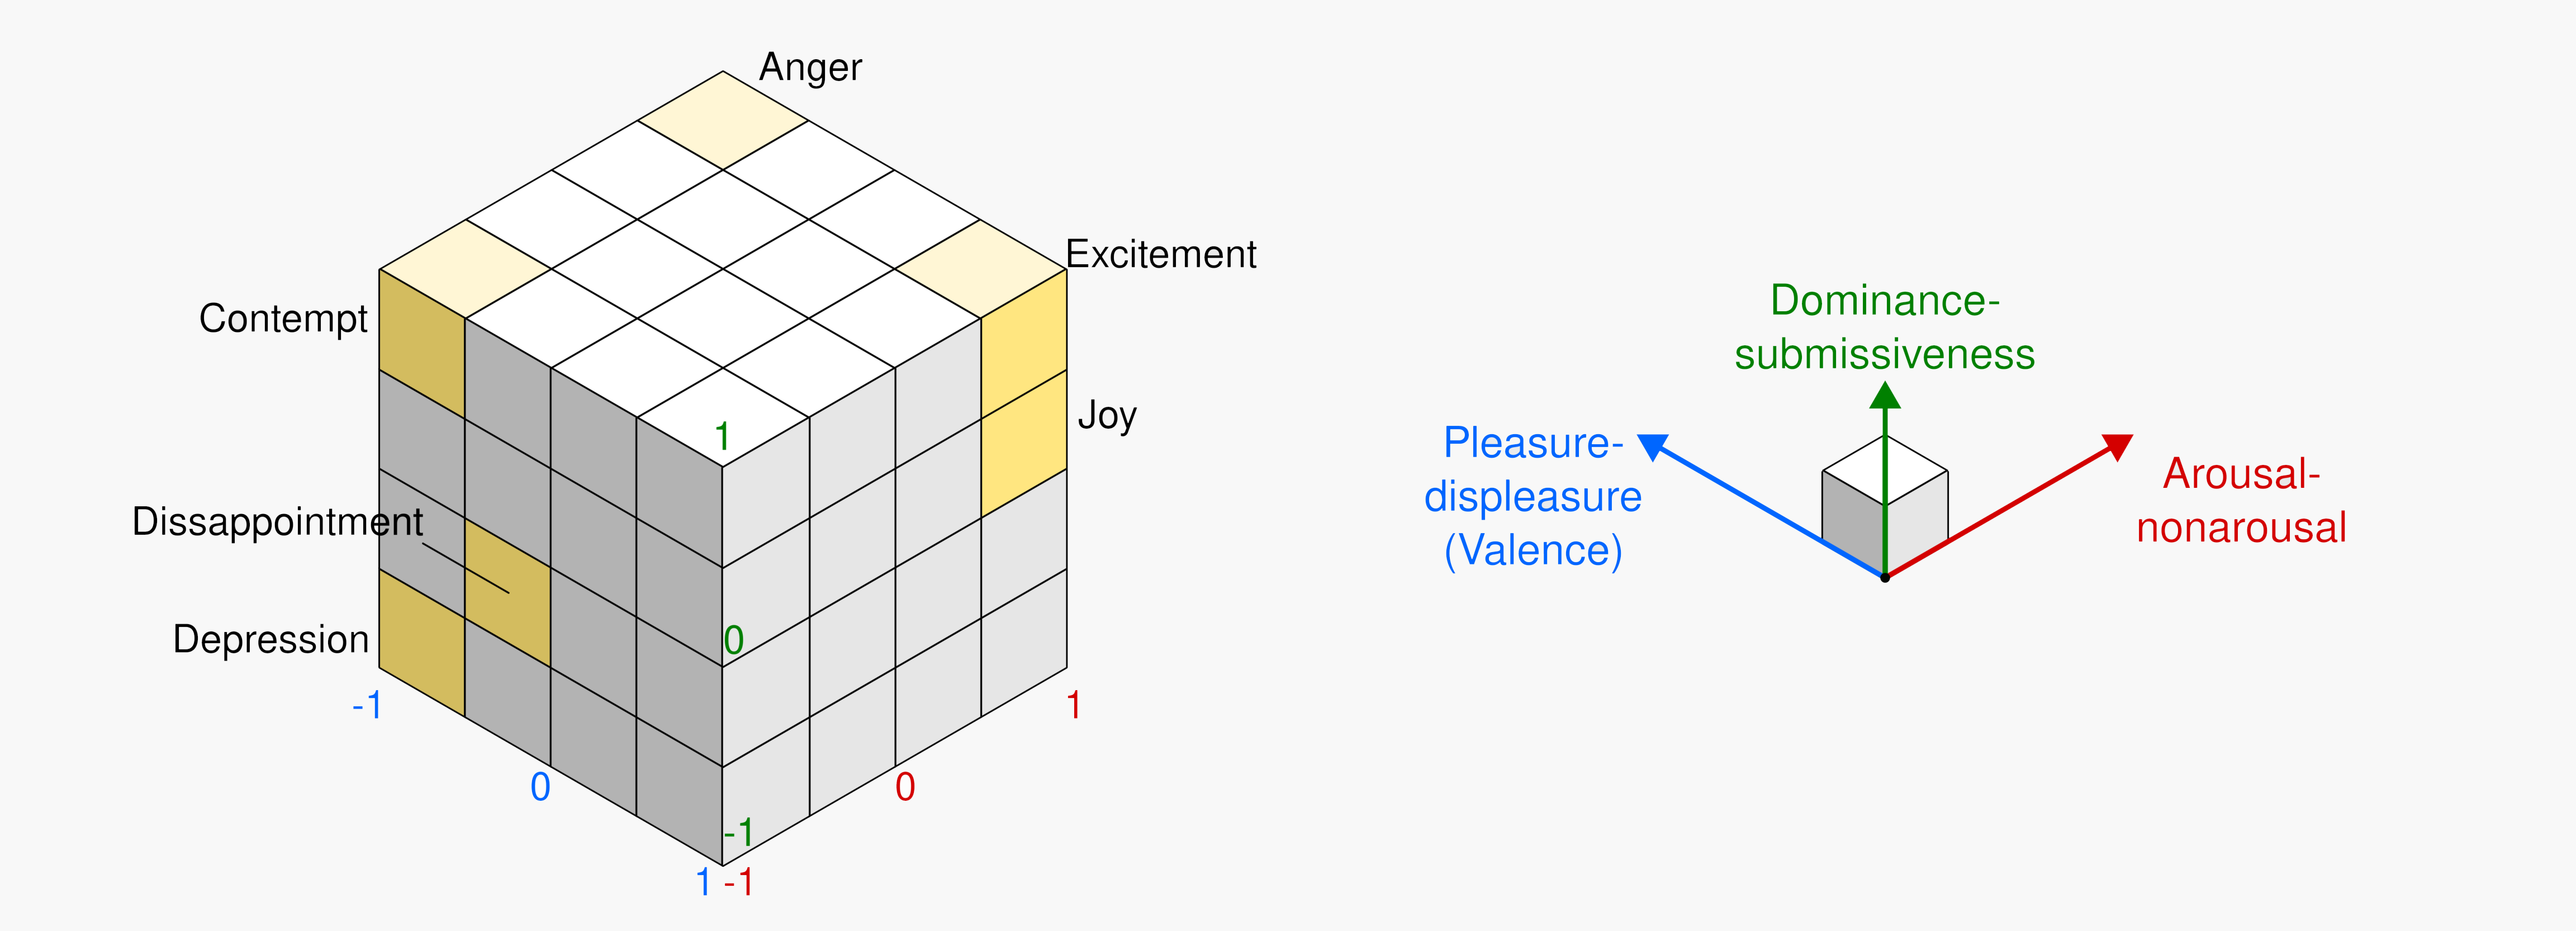
\includegraphics[width=0.8\linewidth]{figures/pad.png}
    \caption{Representation of PAD model done with cubes~\cite{pad}}
    \label{fig:pad}
\end{figure}

Additionally, in the field of affective computing, an explicit attempt to bridge the gap between discrete labels and continuous emotion representations is presented by Buechel et al.~\cite{buechel2021labelagnosticemotionembeddings}. Rather than committing to a single emotion taxonomy, they propose learning \emph{label-agnostic emotion embeddings} that serve as a shared latent representation across heterogeneous annotation schemes, including polarity, basic emotion categories, and affective dimensions such as valence and arousal.

Crucially, emotion labels in this framework are not treated as targets to be predicted directly, but as projections from a common embedding space. Models are trained to map text into this latent affective space, from which multiple label formats can be recovered via lightweight prediction heads. This design enables the learned emotion information to be transferred to another without retraining the full model. Empirically, Buechel et al.\ show that such embeddings preserve prediction quality while supporting cross-dataset generalisation.

Complementary to this, Wang and Zong (2021)~\cite{wang-zong-2021-distributed} focus on learning continuous representations for \emph{emotion categories themselves}. Instead of representing emotion classes as one-hot vectors, they derive distributed emotion embeddings by averaging soft classifier outputs over all instances of a given emotion category. These representations form an emotion space in which distances reflect empirical similarity between emotions as expressed in text. Their results demonstrate that emotion categories cluster by sentiment polarity and intensity, which captures the emotions more faithfully than the conventional semantic word embedding spaces. 

Both of those approaches we looked at enable emotion to be represented as a continuous, low-dimensional structure where each of them corresponds to a region or a direction in a metric space. This perspective aligns closely with psychological theories such as PAD, while remaining grounded in data-driven learning from natural language.

Importantly, representing emotion in continuous spaces shifts the learning problem away from rigid classification toward geometric representation learning. This not only resolves many of the limitations inherent in discrete labels, but also provides a foundation for analysing how emotional information is encoded in vector representations more generally. In particular, it raises the question of whether emotion occupies identifiable subspaces or linear directions within learned embeddings, a topic explored in the following subsection.

\subsection{Linear Structure of Emotion in Word Embedding Spaces} \label{linear_word_embedding}

An important question here is whether the continuous space for emotion is actually reflected in learned language representations. Interestingly, prior to the emergence of LLMs, static word embeddings already exhibited evidence of latent affective organisation, despite being trained without explicit emotional supervision.

Wu and Jiang~\cite{linear_vector_emo} demonstrate that emotional information in word embeddings such as GloVe~\cite{brochier2019global} is not uniformly distributed across dimensions, but instead concentrated along a small number of linear directions. They train a linear autoregressive model to predict continuous emotional valence on annotated narrative data, and show that only a limited subset of embedding dimensions contributes to emotional valence. Interpreting the learned weights reveals that emotional polarity can be captured by a low-dimensional subspace embedded within the full semantic space.

It is also reported that projecting word embeddings into this learned emotion subspace produces a substantially clearer separation between positive and nefative emotion. This indicates that emotion is linearly recoverable even when embeddings are trained without affective objectives. Namely that, emotional meaning is encoded \textbf{geometrically}, rather than a byproduct of lexical associations.

A particularly significant finding is that this projected emotion space preserves \emph{linear compositional structure}. Vector arithmetic over words that contain emotion yields composite affective states, which is also consistent with psychological theories of emotion composition such as Plutchik's wheel of emotions~\cite{plutchik1980emotion}.

\begin{figure}[H]
    \centering
    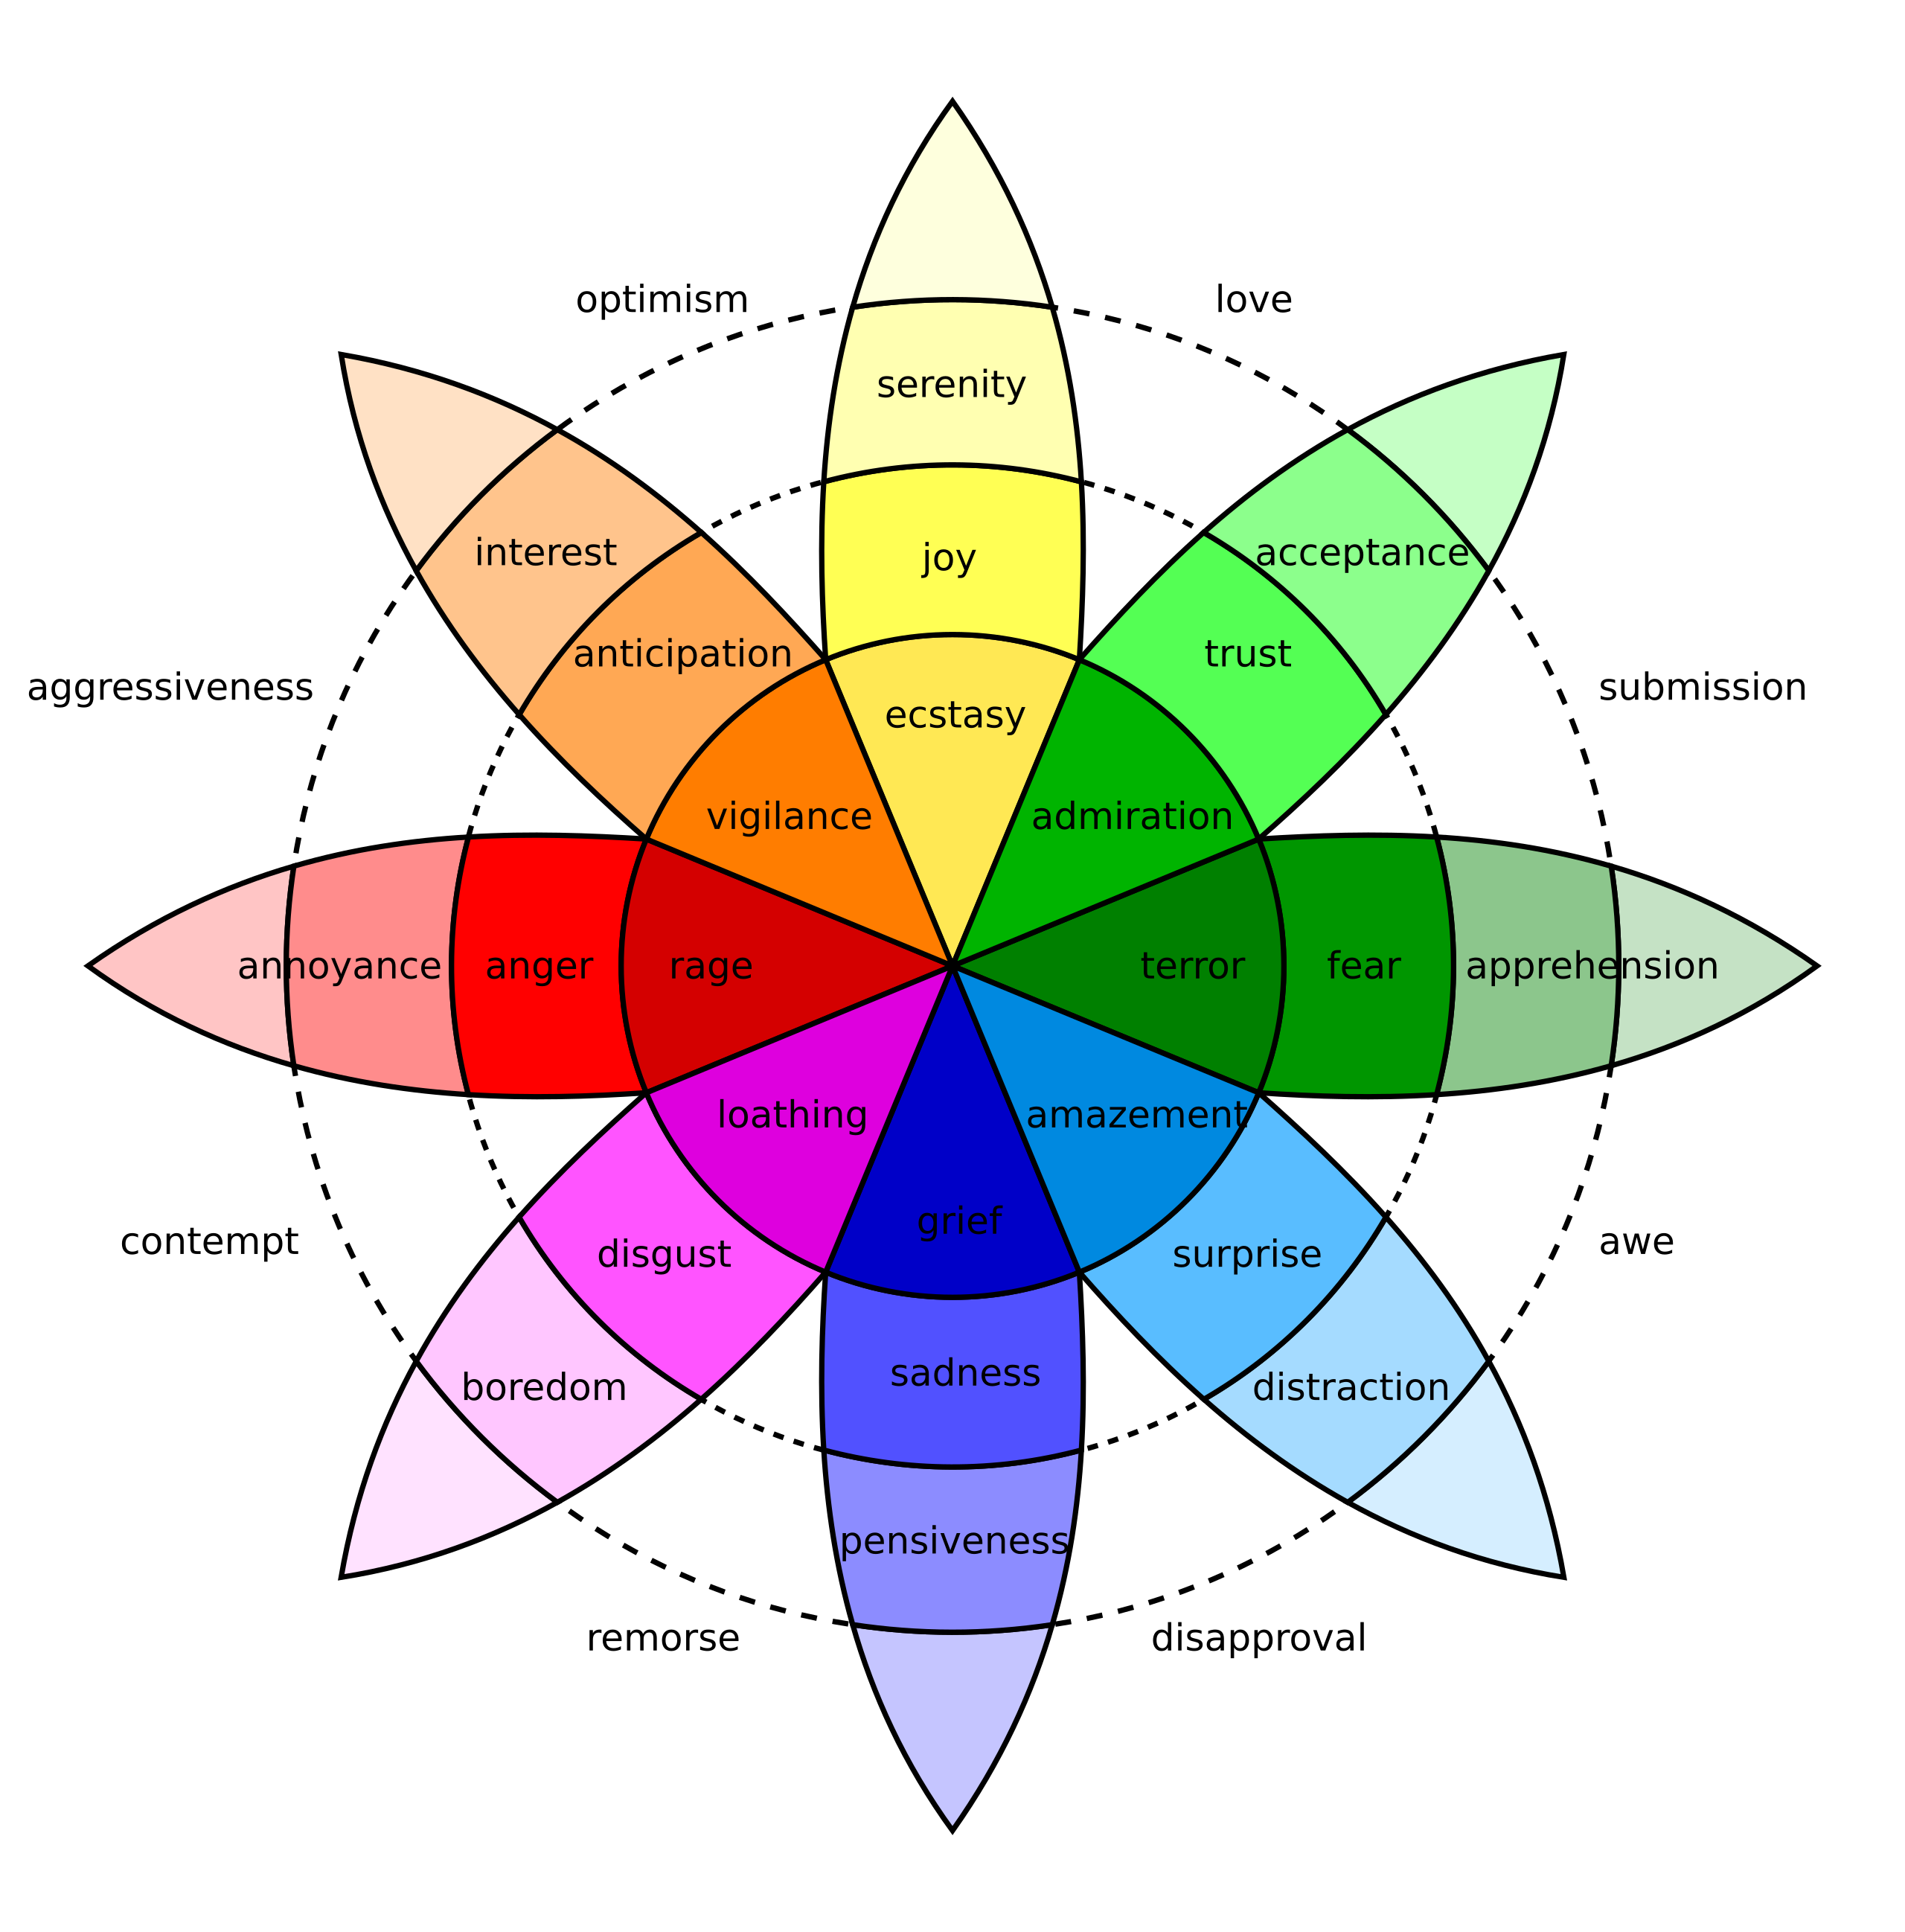
\includegraphics[width=0.5\linewidth]{figures/Plutchik-wheel.png}
    \caption{Plutchik's wheel of emotions: basic emotions are arranged radially, with angular proximity indicating similarity and radial intensity indicating emotional strength.}
    \label{fig:Plutchik}
\end{figure}

For example, the vector sum of \texttt{joy} and \texttt{trust} aligns closely with \texttt{love}, while remaining distant from affectively opposing states such as \texttt{remorse}. This behaviour cannot be captured by categorical representations, but emerges naturally in a continuous, vector-valued framework.

These results indicate that emotion in word embedding spaces is not only continuous but also approximately linear, admitting meaningful projections, directions, and arithmetic operations. As a result, affective similarity, intensity, and composition can be expressed through simple linear operations rather than discrete class boundaries.

Taken together, these findings provide early evidence that emotion is encoded as structured geometry within learned language representations. This establishes a representational bridge between psychological models of emotion and mathematical embedding paradigms. This also motivates further research into how such linear emotional structure scales and evolves in more expressive representation learning systems.

\section{Manipulation of Latent Representations}

To harness these emotion vectors, researchers have explored techniques for directly manipulating internal representations of models.

\subsection{Neuron-Level Emotion Control}

One line of work focuses on exploiting localised affective representations at the neuron level. For instance, Radford et al.\ (2017)~\cite{radford2017learninggeneratereviewsdiscovering} noted a single ``sentiment neuron'' in a byte-level recurrent language model. It has shown that the activation strongly correlates with review polarity and the manipulation of that sentiment neuron directly controls the generated sentiment. Later work shows that modern LLMs contain clusters of neurons selectively responsive to specific emotions. 

Ablation and masking experiments were done by Lee et al.\ (2025)~\cite{lee-etal-2025-large}, and it demonstrates that removing these neurons can selectively impair recognition of particular emotions. This confirms that they play a functional role rather than being incidental correlates. However, there is still a possibility that the model is redundant. For some emotions, performance remains stable after ablation, suggesting overlapping representations and compensatory mechanisms.

Additionally, low-resource fine-tuning methods such as LoRA (Low-Rank Adaptation)~\cite{hu2021loralowrankadaptationlarge} and prefix-tuning operate at a higher level of abstraction but still manipulate latent activations. By injecting small learned vectors into the model we can induce a consistent emotional tone without full retraining. This shows that affective style is encoded in directions that are easy to steer with low-rank updates.

\subsection{Emergent Emotional Subspaces in Large Language Models}

Large language models substantially extend and generalise the affective structure previously observed in static word embeddings (\ref{linear_word_embedding}). Even though models are trained on massive corpora without any emotional information supervision, LLMs acquire rich contextual representations. These models appear to internalise emotion as a continuous and distributed property of their hidden-state geometry.

Recent work provides strong empirical evidence for this claim. Reichman et al.\ (2025)~\cite{reichman2025emotionsartthouunderstanding} show that emotional information in large decoder-only LLMs is organised within a low-dimensional \textbf{emotional manifold} embedded in the activation. 

They analysed hidden states across layers, demonstrated how affective content aligns with a small number of stable latent directions. Importantly, these directions appeared without any explicit emotion supervision, indicating that affective structure is a natural consequence of large-scale language modelling rather than a task-specific artefact. Moreover, the identified emotional subspace is remarkably consistent across domains and languages, suggesting that LLMs internalise a broadly universal affective geometry.

Crucially, this geometry is not merely descriptive. Reichman et al.~\cite{reichman2025emotionsartthouunderstanding} show that small interventions along these latent directions can alter the model's emotional interpretation of an input, while preserving its semantic content. This establishes emotional subspaces as functionally meaningful components of the model's representation space, rather than passive correlates of surface-level sentiment cues. This establishes emotional subspaces to be considered as a functional and meaningful components of the model's representation space.

Complementary evidence comes from neuron-level analyses too. Lee et al.\ (2025)~\cite{lee-etal-2025-large} identify groups of neurons whose activations selectively track specific basic emotions in large instruction-tuned models. Emotional information is broadly distributed, but certain neurons constantly exhibit disproportionately strong responses to particular affective states. Further ablation experiments revealed that suppressing these neurons can significantly degrade emotion recognition performance for some emotions. This provides a causal evidence that emotional information is actively processed rather than epiphenomenal.

Taken together, these findings suggest that emotion in LLMs is best characterised as an emergent, low-dimensional subspace embedded within high-dimensional contextual representations. Emotional meaning is not localised to single units, nor reducible to discrete labels; instead, it occupies a structured region of stable latent space. This emergent affective geometry provides the representational foundation that enables direct control of emotional behaviour through linear interventions, which we discuss next.

\subsection{Steering Latent States with Linear and Continuous Control Vectors}

If emotional meaning in LLMs is encoded as directions or subspaces within latent representations, a natural consequence is that affective behaviour should be directly controllable by intervening along those directions. This observation has motivated a line of work on \textbf{latent steering}, in which linear and continuous control vectors are applied directly to internal activations during inference.

An early and influential approach is Plug-and-Play Language Models (PPLM)~\cite{dathathri2020plugplaylanguagemodels}, combines a frozen language model with an external attribute model (e.g.\ a sentiment classifier) and performs gradient ascent on the hidden states to increase the likelihood of a desired attribute. Effectively, this method introduces a small \textbf{sentiment vector} into the latent representation, biasing generation toward positive or negative emotion without modifying the model's weights. Although originally framed as a controllable generation technique, PPLM implicitly relies on the assumption that affective attributes correspond to approximately linear directions in latent space.

More recent work makes this assumption explicit and removes the need for iterative optimisation. Anthropic's \textbf{Contrastive Activation Addition} (CAA)~\cite{caa} directly intervenes in a model's internal activations using precomputed \textbf{steering vectors}. These vectors are obtained by collecting large sets of positive and negative examples of a target behaviour or attribute and averaging the differences in their intermediate representations. The resulting vector captures a direction in latent space that causally corresponds to the desired attribute. During inference, adding this vector to the residual stream steers model behaviour in a predictable manner, while leaving the model parameters unchanged.

A key advantage of CAA is its simplicity and interpretability. The intervention is linear, and the strength of the effect can be modulated continuously by scaling the steering vector with a scalar coefficient. Moreover, multiple steering vectors can be combined additively, enabling compositional control over several attributes simultaneously. In contrast to prompt engineering or fine-tuning, such interventions operate directly on the model's internal state and often yield more precise and robust control, particularly for abstract properties such as sentiment or emotional tone. 

Crucially, steering latent states does not only affect surface-level lexical choices. Injecting affective control vectors at intermediate layers can alter the model's internal interpretation of emotional context, changing how emotional cues are integrated and propagated through the network. This supports the view that emotion in LLMs functions as a global latent variable, rather than as a property tied to individual tokens or outputs.

As conclusion, latent steering methods such as PPLM and CAA provide strong evidence that emotional subspaces in LLMs are not only emergent and structured, but also causally actionable. Manipulating affective behaviour through simple linear interventions reinforces the interpretation of emotion as a continuous geometric representation space. It further bridges descriptive analyses of emotional geometry with concrete mechanisms for controlling model behaviour.

\subsection{Causal Evidence for Linear Sentiment and Emotion Directions}

The existence of affective directions in representation space can be shown by linear probes or dimension reduction, however, it is still doubtful if they actually play a causal role in model behaviour. Recent work provides strong evidence that emotion directions in LLMs are not only linearly recoverable, but also functionally necessary and sufficient for affective reasoning.

Hollinsworth et al.\ (2024)~\cite{hollinsworth-etal-2024-language} show that sentiment in LLMs is encoded along a single dominant linear direction in contextual embeddings. They perform directional ablations and interventions, demonstrating that removing / suppressing this sentiment direction causes systematic degradation in downstream emotion-sensitive tasks such as emotion classification. Conversely, injecting the same direction into neutral contexts induces predictable shifts in model outputs. This bidirectional manipulation provides an evidence that the emotion direction is actively used by the model rather than being a passive correlate.

Importantly, affective competence in LLMs does not depend on explicit fine-tuning for emotion-related tasks. Broekens et al.\ (2023)~\cite{broekens2023finegrainedaffectiveprocessingcapabilities} demonstrate that off-the-shelf LLMs such as ChatGPT can map text to precise valence–arousal–dominance (VAD) values and detect fine-grained emotional cues using prompting alone. This sugegsts that continuous affective representations are already embedded in the latent space as part of general language understanding. This is a strong evidence that interpretes emotion as a pre-verbal latent variable, rather than a task-specific output format.

At larger scales, evidence further indicates that emotional representations are not flat but hierarchically structured. Zhao et al.\ (2024)~\cite{zhao2025emergencehierarchicalemotionorganization} observe that very large models (more than 405 billion parameters) develop tree-like emotion representations, where basic affective states branch into more specific emotions. Models featuring a more consistent hierarchical affective geometry demonstrate enhanced emotion recognition capabilities and increased persuasive effectiveness in negotiation scenarios. This directly links the internal structure of emotional expression to functional behaviour.

These findings converge on a causal interpretation of affective geometry in LLMs. Removing emotion directions impairs affective reasoning, while injecting them predictably alters behaviour. Moreover, emotional information is not confined to isolated tokens or neurons, but is accumulated and summarised across layers into global latent variables that shape general affective capabilities of models.

In conclusion, there is a principled foundation for vector-based manipulation of emotion, which enables us to express emotional nuance through numeric operations on embeddings rather than token-level substitutions. This causal grounding is essential for our project that seeks to control and align emotional behaviour in large language models.

\section{Reasoning Beyond Token Space}

\subsection{Limitations of Token-Based Reasoning}

Conventional LLMs reason in token space. Because inputs are projected onto the discrete boundaries humanity drew as ``vocabulary,'' fine affective nuance and embodied subtleties are irretrievably lost during that projection, and what remains in one output language may differ from what remains in another. To adjust tone, one often uses prompt engineering or instruction tuning (``Please answer politely,'' etc.), but adherence is uncertain and fine-grained control is difficult. Other countermeasures include supervised fine-tuning to internalise a style, or label-conditioned generation (e.g.\, adding \texttt{<joy>} \texttt{<sad>}), but fine-tuning is costly and switching between styles is inflexible; label conditioning also cannot capture complex blends of nuance.

Beyond affective control, the same limitation applies to reasoning itself. Autoregressive language models do not take token functionality into account in its generation process. Even if the token carries significant reasoning content, it will be allocated approximately same computational budget as grammartical tokens like \texttt{a} or \texttt{is}. As a result, only a small subset of internal states carries the actual inferential work, and most of the tokens in explicit reasoning traces do not contribute to the underlying computation.

Recent works show this disconnectivity between the surface output tokens and internal reasoning process. Pfau et al.\ (2024)~\cite{pfau2024lets} demonstrate that transformers can perform non-trivial hidden computation even when output tokens are semantically uninformative. For example, inserting filler or pause tokens (carry no explicit meaning) somehow measurably improve performance on reasoning tasks. This suggests that the essential computation is carried by latent activations rather than by the emitted tokens themselves. Token generation only a communicative language constraint around an internal process.

The inefficiency of token-based reasoning becomes more apparent when reasoning is explicitly verbalised. Chain-of-thought prompting improves performance in many tasks, however \textbf{it requires the model to externalise intermediate states into natural language, even when those states are not naturally linguistic}. As argued by Hao et al.\ (2025)~\cite{hao2025traininglargelanguagemodels}, language is optimised for communication rather than for computation. Forcing reasoning to unfold within the constraints of a discrete vocabulary introduces unnecessary overhead and distortion. Many reasoning tokens exist not because they are required for inference, but because they are required for human readability.

From this perspective, explicit verbalisation constitutes a form of lossy compression for an affective reasoning as discussed in the previous section. The continuous and high-dimensional internal states during inference must be projected onto a discrete and culturally contingent token space, which flattens distinctions that are visible for computation but words-level invisible. This compression is problematic for affective computing, because emotion structure is inherently graded, which is resistant to precise lexicalisation.

Taken together, these observations suggest that token space not a substrate of reasoning, but rather an interface. While it provides a convenient medium for communication and supervision, it is suboptimal for internal computation. This motivates a growing line of work that seeks to decouple reasoning from explicit token generation. Computation can proceed without the constraints imposed by language.

\subsection{Reasoning in Continuous Latent Space}

Motivated by the observation that reasoning is primarily carried by latent activations rather than surface tokens, a growing body of work has explored \textbf{implicit} forms of chain-of-thought. The central idea is to retain the intermediate reasoning within the model's hidden state, so that we can benefit from the multi-step reasoning while avoiding the distortions introduced by forcing intermediate states into natural language.

Early implicit chain-of-thought approaches aim to internalise reasoning traces by gradually removing explicit reasoning tokens during training, encouraging the model to perform the same computation silently in its latent space. More recent methods go further by explicitly allocating computation to continuous latent representations that replace textual reasoning steps altogether. In these models, reasoning unfolds as a sequence of hidden-state transitions, while the output layer is used only to produce the final answer.

A representative work is \textbf{CODI} (Compressing Chain-of-Thought into Continuous Space via Self-Distillation)~\cite{shen2025codicompressingchainofthoughtcontinuous}. This approach compresses explicit chain-of-thought trajectories into a compact sequence of continuous latent states, and by distilling a teacher model that produces explicit reasoning traces, CODI trains a student model to reproduce the same reasoning outcome using a shorter sequence of latent vectors. This demonstrates that the information carried by textual reasoning can be encoded more efficiently in continuous space, without requiring token-level supervision at inference time.

A more radical approach is proposed by \textbf{Coconut} (Chain of Continuous Thought)~\cite{hao2025traininglargelanguagemodels}. Rather than compressing explicit reasoning traces, Coconut modifies the inference procedure itself by feeding the model's last hidden state back as the next input embedding. In this way, reasoning unfolds entirely within continuous latent space and there is no need of intermediate textual tokens at all. However, because Coconut relies primarily on answer-level supervision, the resulting latent trajectories can be unstable when extended to deeper reasoning chains, which we discuss in the next subsection.

\subsection{Implicit and Continuous Chain-of-Thought}

However, there is one challenge that purely implicit reasoning introduces. When multiple latent reasoning steps are chained together without sufficient structural constraints, the latent representations can collapse into homogeneous states. This phenomenon is often referred to as \textbf{latent collapse}, which undermines the model's ability to maintain distinct intermediate representations.

\textbf{SIM-CoT} (Supervised Implicit Chain-of-Thought)~\cite{wei2025simcot} addresses this limitation by introducing step-level supervision during training. Instead of supervising only the final answer or the overall reasoning trajectory, SIM-CoT attaches an auxiliary decoder that forces each latent reasoning step to predict a corresponding explicit reasoning phrase. This alignment ensures that each latent vector encodes distinct, semantically meaningful content, preventing homogenisation and improving stability. Crucially, the auxiliary decoder is used only during training and is removed at inference, allowing the model to retain the efficiency of silent latent reasoning while benefiting from structured supervision. Empirically, SIM-CoT substantially improves both performance and robustness over earlier latent reasoning models, including Coconut-style architectures.

It attaches an auxiliary decoder that forces each latent reasoning step to predict a corresponding explicit reasoning phrase, which ensures that each latent vector to encoded semantically meaningful content. This substantially improves both performance and robustness over earlier latent reasoning models, including Coconut-style architectures. Importantly, the auxiliary decoder is used only during training and is removed at inference, allowing the model to retain the efficiency of silent latent reasoning while benefiting from structured supervision.

These approaches demonstrate that chain-of-thought need not be realised as a sequence of discrete tokens. Reasoning can be instead implemented as a controlled trajectory through continuous latent space, with explicit language serving primarily as a training scaffold or interpretability aid.  Implicit and continuous chain-of-thought models provide a natural foundation for studying how emotions may be represented and manipulated within latent reasoning processes.

\subsection{Implications for Affective Representation}

The developments reviewed above suggest a converging picture of representation and computation in LLMs. As discussed in earlier sections, emotions are not confined to discrete labels or lexical choices but it rather emerges as a continuous structure within latent space. At the same time, recent advances in implicit chain-of-thought demonstrate that reasoning itself can be implemented as a trajectory through that same latent space, without requiring intermediate symbolic tokens.

These findings summarises to the fact that emotion need not be treated as separate components at the level of surface language. Instead, it appears to be grounded in shared latent representations that evolve over the course of inference. From this perspective, emotional information may constitute an integral part of the internal reasoning state itself, shaping how intermediate representations are formed and propagated.

Importantly, this possibility remains largely unexplored. Although latent reasoning frameworks have demonstrated improved eff expressivity for logical and mathematical tasks, their implications for affective representation have not been systematically examined. Whether emotional dimensions align or interact with latent reasoning trajectories is an open question. Addressing this gap requires moving beyond token-level analysis and considering emotion as a first-class component of latent computation rather than as a stylistic attribute.

These considerations motivate the investigation in the following chapters. Rather than treating emotion as an external label or an output constraint, we explore the hypothesis that affective states can be represented within continuous latent spaces that underlie reasoning itself. By doing so, we aim to better understand how emotional meaning may be re-expressed when language is no longer the primary medium of inference.

%%%%%%%%%%%%%%%%%%%%%%%%%%%%%%%%%%%%
\chapter{Affective Steering Pipeline}
\label{chap:development1_emo_steering}

This chapter demonstrates that contrastive activation addition (CAA) vectors can be constructed in the emotion context of a large language model, and that these vectors decompose naturally into a \textbf{shared emotionalisation component} and an \textbf{emotion-specific residual component}. The central empirical finding is that only the residual component is needed for reliable affective steering.

\section{Chapter Roadmap}
\label{sec:steering_roadmap_1}
This chapter proceeds through five stages that build toward that claim.

\begin{enumerate}
  \item \textbf{Prerequisites}: Before computing CAA vectors, three building blocks are required. Firstly we need a controlled dataset of emotional rewrites paired with neutral paraphrases. Then, residual-stream activations are extracted from the model, and a principled layer is selected to identify which transformer layer best abstracts pre-verbal affective structure. These are covered in Sections~\ref{sec:dataset_construction},~\ref{sec:residual_extraction}, and~\ref{sec:layer_selection}.

  \item \textbf{CAA vector construction} (Section~\ref{sec:caa_construction}): Using the extracted activations, we compute contrastive vectors for each emotion by averaging the difference between emotion-conditioned and neutral-conditioned hidden states across source texts and intensity levels.

  \item \textbf{Observation}: Inspecting the inter-emotion cosine similarities of the resulting CAA vectors reveals a striking pattern; all pairs of emotion vectors lie in the range $0.91$--$0.97$. This near-uniformity indicates that the vectors are \textbf{dominated by a shared direction activated regardless of the target emotion}, and directly motivates the decomposition introduced next.

  \item \textbf{Decomposition} (Section~\ref{sec:decomposition}): We define a shared emotionalisation vector $\mathbf{g}$ as the normalised mean of all emotion CAA vectors, and project it out by orthogonal projection to obtain emotion-specific residual vectors $\hat{\mathbf{r}}_e$. The resulting two-component steering parameterisation is
  \[
    \Delta_e(\alpha_G,\alpha_R)=\alpha_G\,\mathbf{g}+\alpha_R\,\hat{\mathbf{r}}_e,
  \]
  where $\alpha_G$ controls global emotionalisation strength and $\alpha_R$ controls emotion-specific directionality.

  \item \textbf{Steering evaluation} (Section~\ref{sec:steering_experiments}): We test whether adding this intervention at inference time reliably shifts generated text toward the target emotion, and sweep over $(\alpha_G, \alpha_R)$ to find the best operating point. The key finding is that including the shared component $\mathbf{g}$ ($\alpha_G > 0$) does not improve and is in fact slightly counterproductive. The practical conclusion is to discard $\mathbf{g}$ and steer with the residual alone ($\alpha_G \approx 0$, $\alpha_R > 0$).
\end{enumerate}

\section{Dataset Construction}\label{sec:dataset_construction}

In order to investigate whether emotion is encoded as structured geometry in residual space, we constructed controlled rewrite datasets from shared source utterances. The primary dataset is an emotion-category rewrite set derived from two dialogue corpora: DailyDialog~\cite{li2017dailydialogmanuallylabelledmultiturn} and EmpatheticDialogues~\cite{rashkin2019empatheticopendomainconversationmodels}. We selected dialogue data because conversational utterances provide compact emotional signals grounded in context in everyday interpersonal situations, while keeping propositional content sufficiently constrained for controlled rewriting. For each source utterance, we used GPT-4.1-mini to generate rewrites for Plutchik's eight basic emotions (joy, trust, fear, surprise, sadness, disgust, anger and anticipation) at three matched intensity levels (low, medium and high). This yields $8\times3 = 24$ affective variants per source text. A central constraint throughout the construction process was to preserve meaning: the underlying situation and factual content were held constant while only the affective framing was systematically varied.

\begin{table}[H]
\centering
\small
\begin{tabular}{p{0.12\linewidth} p{0.82\linewidth}}
\toprule
\textbf{Emotion} & \textbf{Utterance} \\
\midrule
\textbf{Base} & \textbf{I waited for hours and nobody came.} \\
Joy & Nobody came for hours, but I ended up enjoying the quiet time on my own. \\
Trust & Nobody came for hours, but I am sure they had a valid reason. \\
Fear & Nobody came for hours, and I started worrying that something might have gone wrong. \\
Surprise & Nobody came for hours, and honestly I did not expect that at all. \\
Sadness & For hours, nobody came. I guess that says enough. \\
Disgust & Nobody came for hours; that felt deeply inconsiderate. \\
Anger & Nobody came for hours, and I am really frustrated about wasting all that time. \\
Anticipation & Nobody came for hours, but I kept thinking they might still arrive any minute. \\
\bottomrule
\end{tabular}
\caption{Illustrative rewrites for all eight Plutchik emotion categories at matched medium intensity.}
\label{tab:emotion_rewrite_example}
\end{table}

As a control condition, we constructed an additional neutral paraphrase baseline dataset. In this dataset, each source utterance has been rewritten into an affectively neutral but semantically equivalent form. This baseline provides a reference representation of content without targeted emotional colouring, enabling contrastive analysis between emotion-conditioned and emotion-suppressed activations. \par

\begin{table}[H]
\centering
\small
\begin{tabular}{p{0.22\linewidth} p{0.72\linewidth}}
\toprule
\textbf{Field} & \textbf{Example} \\
\midrule
Base utterance & What a mess!  Sorry. I'll clean it up. \\
Neutral paraphrase & There is a mess. I will clean it up. \\
\bottomrule
\end{tabular}
\caption{Illustrative example from the neutral-paraphrase control dataset.}
\label{tab:neutral_rewrite_example}
\end{table}

Together, these datasets enable us to distinguish emotional signals from lexical-semantic content. This provides an empirical basis for the decodability, geometry and steering analyses presented in subsequent sections.\par

This design makes it possible to ask whether affective variation forms a consistent vector in activation space, rather than merely reflecting surface-level lexical differences between emotional words.\par

%TODO: dataset size

\section{Residual-Stream Extraction}
\label{sec:residual_extraction}

We extract hidden-state activations from an instruction-tuned language model (Llama-3.1-8B~\cite{meta2024llama318b}) with no gradient updates. We use the HuggingFace Transformers library~\cite{wolf2020huggingfacestransformersstateoftheartnatural} to implement the forward pass and activation extraction.

To ensure that the inputs are comparable across the different conditions, each sample is formatted with a shared instruction prefix that is constructed from the same base utterance. Only the continuation text is changed, either through an emotion rewrite or a neutral paraphrase. Specifically, we use a user instruction in the form of a chat template that asks for a rewrite aligned with the speaker's feelings, and then append the rewritten sentence as the assistant continuation. This matching protocol controls for variance at the prompt level and enables direct comparison of emotion-conditioned and neutral-conditioned activations.

\begin{table}[H]
\centering
\label{tab:activation_prompt}
\begin{tabular}{p{0.95\linewidth}}
\toprule
\textbf{Template Prompt} \\
\midrule
Please rewrite this so it aligns with my feelings more. \\
Start straight from the rewritten text without any preamble, and only provide \textbf{one} rewritten version. \\
Base: \texttt{\{base\_text\}} \\
\bottomrule
\end{tabular}
\caption{Prompt format used for activation extraction.}
\end{table}

Figure~\ref{fig:residual_extraction} illustrates the process of residual stream extraction during a forward pass. The prompt containing both user and assistant tokens is passed through the transformer stack, and hidden states are recorded at selected layers. Each transformer block updates the residual stream through attention and MLP sublayers, producing layer-wise activations $h^\ell \in \mathbb{R}^{T \times d_\text{model}}$, where $T$ is the number of tokens and $d_\text{model}$ is the hidden dimension. 

\begin{figure}[H]
    \centering
    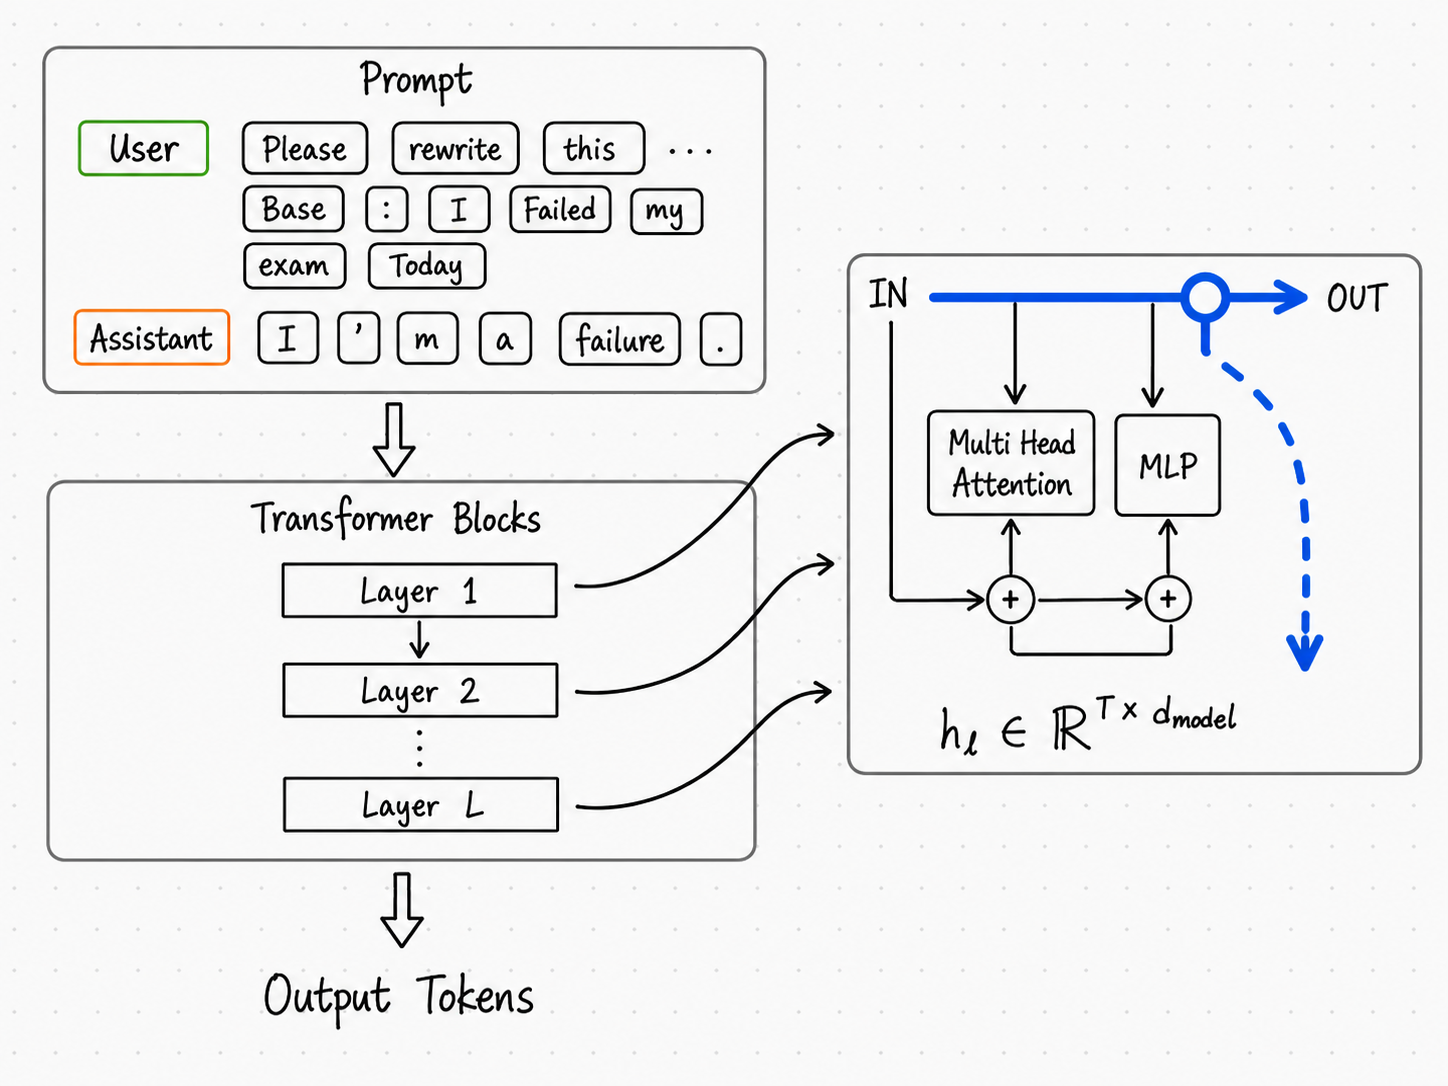
\includegraphics[width=0.6\linewidth]{figures/residual_extraction.png}
    \caption{Schematic overview of residual stream extraction during a forward pass. Tokenisation process is simplified for clarity. In reality, the input is tokenised into subword units e.g. ``please'' might be tokenised into ``ple'' and ``ase''.}
    \label{fig:residual_extraction}
\end{figure}

For each target layer $l$, the last token's hidden state is taken from the layer's output, i.e.
\[
\mathbf{h}_{l}=\texttt{hidden\_states}[l+1][:,-1,:]
\] 
Since tokenisation uses left padding, the index $-1$ consistently corresponds to the \textbf{final} real token in each sequence in the batch. Final-token representation is the state after the model has processed the entire rewritten utterance, making it a compact summary of the affective framing expressed by the continuation. Activations are sampled from layers $\{8,10,13,16,19,22\}$, producing a multi-layer representation for every input.

In summary, the emotion-intensity extraction pipeline produces a 5D tensor:
\[
\mathbf{H}^{\text{emo}} \in \mathbb{R}^{N \times E \times I \times L \times D},
\]
where $N$ is the number of source texts, $E=8$ emotions rewrites, $I=3$ intensity levels, $L$ is the number of sampled layers, and $D=4096$ is the hidden dimension. The neutral baseline pipeline produces:
\[
\mathbf{H}^{\text{neu}} \in \mathbb{R}^{N \times L \times D}.
\]
Source IDs are sorted to align both tensors by index, allowing direct subtraction
\[
\Delta\mathbf{H}_{n,e,i,l,:}=\mathbf{H}^{\text{emo}}_{n,e,i,l,:}-\mathbf{H}^{\text{neu}}_{n,l,:},
\]
which isolates affective shifts while controlling for base semantic content.

\section{Layer Selection and Diagnostics}
\label{sec:layer_selection}

Not all transformer layers provide equally useful representations for affective analysis. Emotion-related structure may be present at multiple depths, but different layers can privilege different properties of the representation. As described in the Roadmap~\ref{steering_roadmap_1}, the aim of the layer selection stage is to identify the layer where emotion before verbalisation are best abstracted. For example, one layer may provide strong emotion-category separability, while another may better preserve a compact low-dimensional geometry. We define three diagnostic metrics to evaluate candidate layers:

\begin{enumerate}
  \item \textbf{Balanced Accuracy}: This metric measures if that layer preserves the emotion category information. We train a logistic regression model to predict the emotion category from the residual vectors, which are PCA-ed into a 4D subspace. The higher this value is, the more our residual space possesses a structure that can be linearly mapped to human-named emotion labels.
  \item \textbf{Geometric Compactness}: This shows if the emotion information is concentrated in a low-dimensional subspace. We measure the explained variance ratio (EVR) of the emotion centroids in the residual space. This metric assesses to what extent the few principal components extracted by PCA/SVD can explain the variance in the original residual vector set.
  \item \textbf{Graded Affect Sensitivity}: This metric quantifies whether the representation of that layer merely ``separates emotion categories'' or whether it possesses ``emotional quantity, and intensity'' as continuous variables. By performing PCA for each emotion label and projecting all samples onto the vector with the greatest variance within each emotion (PC1), we obtain coordinates indicating the position of each sample on the PC1 axis. The Spearman correlation between this score and the intensity label (low, medium, high) serves as a measure indicating that the vector of greatest variation within that emotion aligns with the intensity level. This is then averaged across the eight emotions.
\end{enumerate}

\begin{table}[H]
\centering
\small
\begin{tabular}{lccc}
\toprule
\textbf{Layer} &
  \textbf{Balanced Acc} &
  \textbf{EVR\textsubscript{4}} &
  \textbf{Graded Affect Sensitivity} \\
  & \textit{(4-D subspace)} & & \\
\midrule
  8  & 0.6914 & 0.8834 & 0.1312 \\
  10 & 0.6751 & 0.8876 & 0.0998 \\
  13 \textbf{*} & \textbf{0.7033} & 0.8920 & \textbf{0.1336} \\
  16 & 0.6704 & \textbf{0.8958} & 0.1297 \\
  19 & 0.6198 & 0.8902 & 0.1142 \\
  22 & 0.6142 & 0.8928 & 0.1022 \\
\bottomrule
\end{tabular}
\caption{Layer-wise diagnostic summary for candidate layers. Emotion-category probe balanced accuracy (4-D subspace), centroid compactness (EVR\textsubscript{4}), and mean local intensity-vector correlation. Bold indicates the best value per column; asterisk marks the selected reporting layer.}
\label{tab:layer_diagnostics}
\end{table}

Based on these diagnostics, layer 13 was selected as the primary layer for the main analyses. It is not globally best on every metric, but it provides the most convincing overall trade-off between the above three criteria.

\begin{figure}[H]
    \centering
    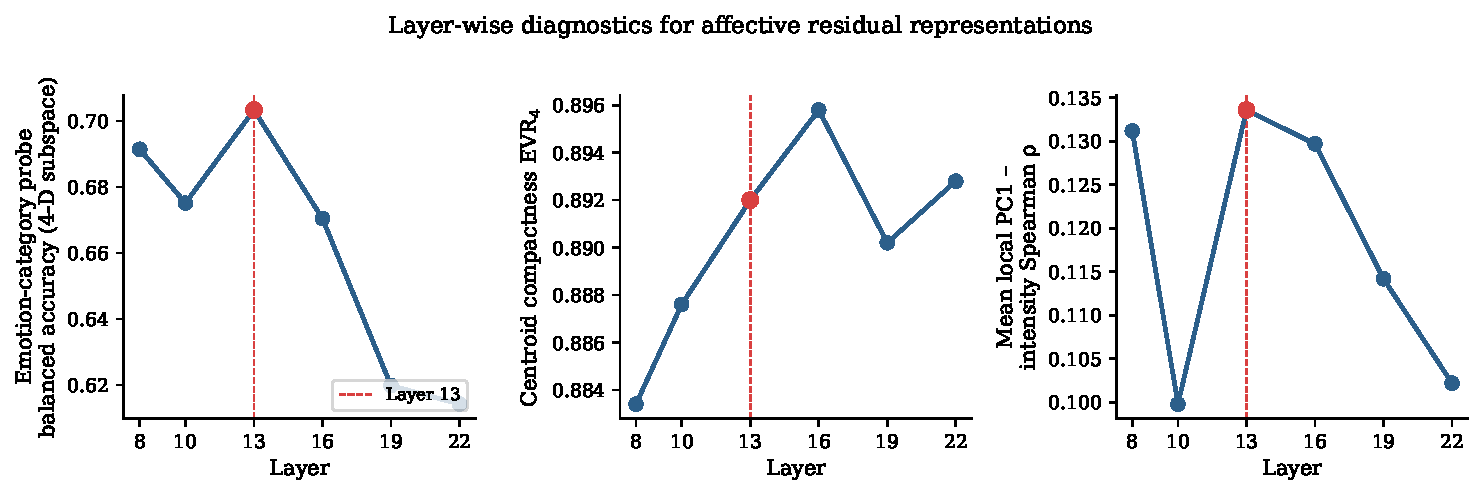
\includegraphics[width=0.8\linewidth]{figures/layer_diagnostics_lineplot.pdf}
    \caption{A visualisation of the layer diagnostics across candidate layers.}
    \label{fig:layer_diagnostics}
\end{figure}

Firstly, \textbf{layer 13 achieves the highest balanced accuracy of all the candidate layers}. Balanced accuracy reaches $0.7033$ in the residual subspace, compared to $0.6914$ in layer 8, $0.6751$ in layer 10 and $0.6704$ in layer 16. This suggests that the emotional representation in layer 13 can be most easily converted into human-named emotion categories, even after compression into a small number of dimensions. However, this does not necessarily mean that the model represents emotions as discrete symbolic labels. Rather, it indicates that the continuous affective geometry at this layer is organised in such a way that human emotion categories can be identified using a simple linear classifier.\par

Secondly, \textbf{layer 13 preserves a highly compact, low-dimensional geometry}. Its centroid-level $\mathrm{EVR}_{4}$ is $0.8920$, meaning that the top four principal components explain $89.2\%$ of the variance among the emotion centroids. Although layer 16 has the highest $\mathrm{EVR}_{4}$ value ($0.8958$), the difference between layers 13 and 16 is small. Therefore, the stronger category decodability at layer 13 does not appear to result in a loss of the low-dimensional affective structure. In this sense, layer 13 preserves a geometry that is both compact and interpretable.\par

Thirdly, \textbf{layer 13 shows the highest graded affect sensitivity of all the tested layers}. The mean intensity-vector correlation is $0.1336$ at layer 13, compared to $0.1312$ at layer 8, $0.0998$ at layer 10 and $0.1297$ at layer 16. As the absolute value is modest, we do not interpret the local PC1 of each emotion as a pure intensity axis. Instead, this metric should be interpreted as an indication of whether the dominant variation within each emotion retains some monotonic relationship with affective strength. The fact that layer 13 achieves the highest value suggests that it preserves slightly more graded affective information than neighbouring layers.\par

Taken together, these diagnostics suggest that layer 13 is close to a useful abstraction point for pre-verbal affective structures. Earlier layers, such as layers 8 and 10, retain substantial affective information, but their category recoverability and graded sensitivity are weaker or less stable. Later layers, such as layer 16, have a marginally more compact geometry but show lower emotion-category balanced accuracy. This indicates that later representations are shaped by subsequent verbalisation. Therefore, layer 13 offers the best overall trade-off: it is low-dimensional enough to support geometric analysis and linearly organised enough to recover human emotion labels. It is also sensitive enough to retain graded affective variation.\par

We therefore use layer 13 as the primary reporting layer in subsequent analyses. However, we do not treat it as the only layer at which affective structure exists. Neighbouring layers show similar trends, indicating that the affective geometry is distributed across multiple middle layers rather than being localised to a single transformer block. Layer 13 should be understood as the most suitable operational layer for this study, i.e. the layer at which the representation is most useful for modelling emotion before it is collapsed into explicit verbal labels.\par

\section{CAA Vector Construction}
\label{sec:caa_construction}

\begin{figure}[H]
    \centering
    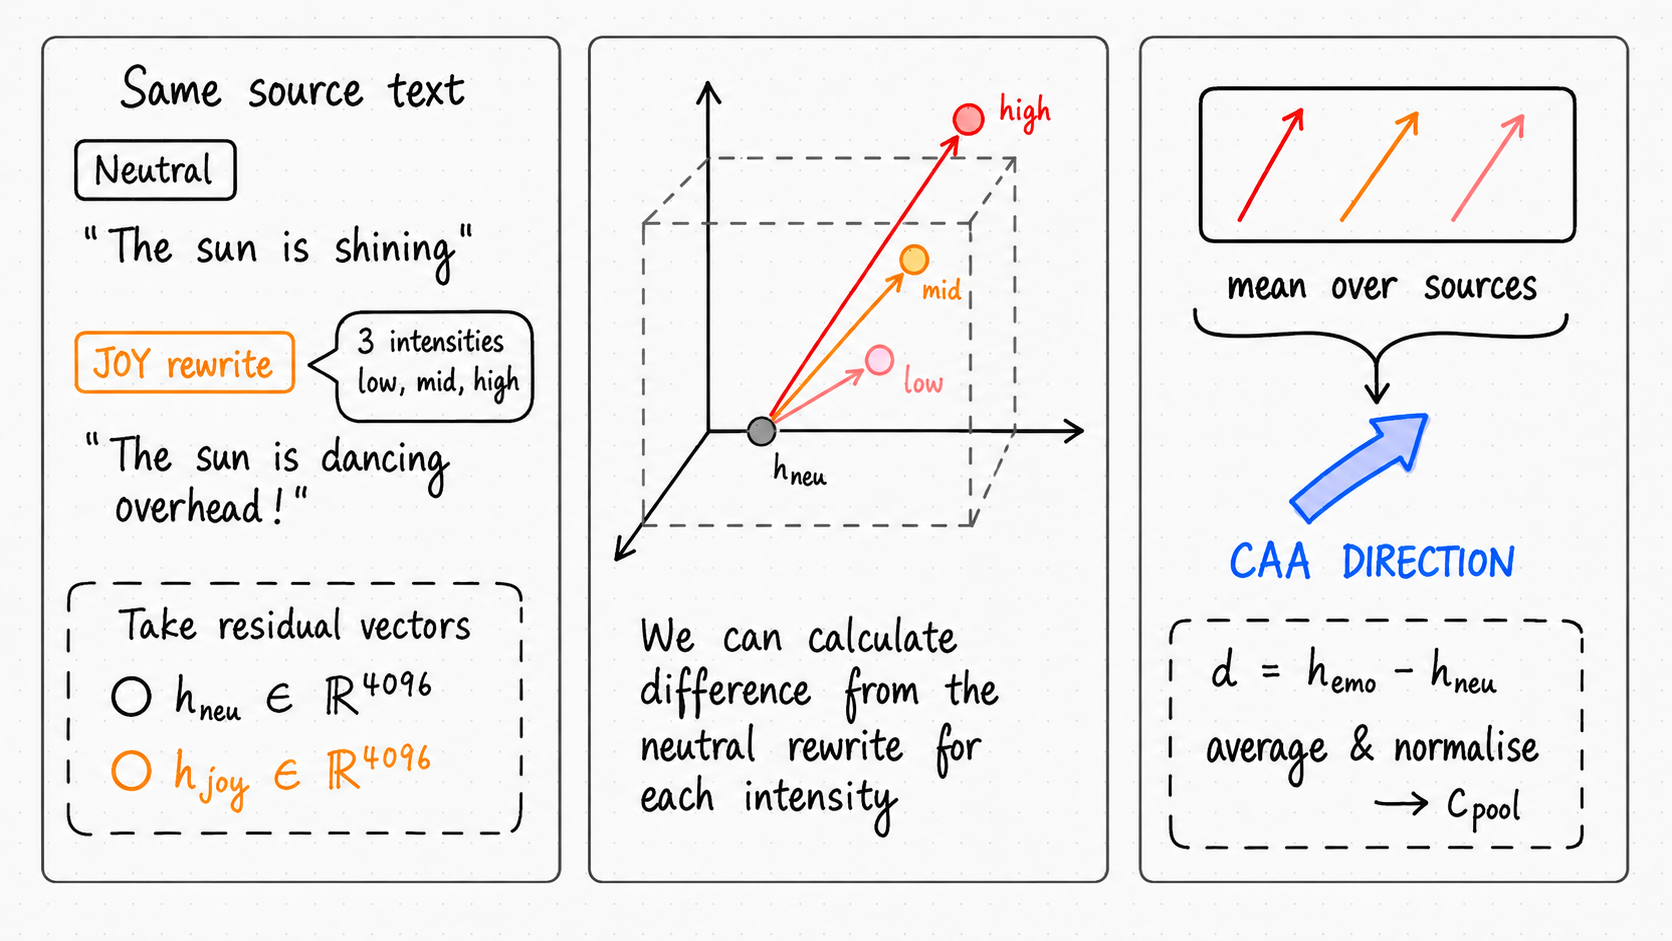
\includegraphics[width=0.6\linewidth]{figures/caa_construction.png}
    \caption{Schematic overview of CAA vector construction.}
    \label{fig:caa_construction}
\end{figure}

In order to convert contrastive residual differences into controllable steering signals, we derive Contrastive Activation Addition (CAA) vectors from emotional and neutral conditioned activations. For each source utterance $n$, emotion $e$, intensity level $i$, and layer $l=13$, we first define
\[
\Delta_{n,e,i,l}=\mathbf{h}^{\mathrm{emo}}_{n,e,i,l}-\mathbf{h}^{\mathrm{neu}}_{n,l}.
\]
We then average over sources and normalise to unit length:
\[
\bar{\Delta}_{e,i,l}=\frac{1}{N}\sum_{n=1}^{N}\Delta_{n,e,i,l},
\qquad
\mathbf{c}_{e,i,l}=\frac{\bar{\Delta}_{e,i,l}}{\lVert\bar{\Delta}_{e,i,l}\rVert_2}.
\]
The vectors $\mathbf{c}_{e,i,l}$ are intensity-specific CAA vectors.

As the steering stage primarily targets the emotional category, treating intensity as a secondary modulation, we also build \textbf{mean emotion vector} $\mathbf{c}^{\mathrm{pool}}_{e,l}$ by averaging across intensities and re-normalising:
\[
\mathbf{c}^{\mathrm{pool}}_{e,l}
=
\frac{\frac{1}{I}\sum_{i=1}^{I}\bar{\Delta}_{e,i,l}}
{\left\lVert\frac{1}{I}\sum_{i=1}^{I}\bar{\Delta}_{e,i,l}\right\rVert_2}.
\]

In the main steering analyses, these pooled unit vectors are used as the primary candidate steering vectors. \par

Figure~\ref{fig:caa_construction} illustrates the construction process. For each emotion and intensity, we compute the mean contrastive shift across sources, and then normalise to obtain a unit vector. The pooled vector is obtained by averaging the intensity-specific vectors and re-normalising. This process yields a set of emotion-specific CAA vectors that can be used for steering interventions.\par

We first confirm that the construction is stable: at layer 13, mean cosine similarity between per-source contrastive shifts $\Delta_{n,e} = h^\text{emo}_{n,e} - h^\text{neu}_n$ and the global CAA vectors $\mathbf{c}^\text{pool}_{e,13}$ ranges from $0.8536$ to $0.8570$ (standard deviation $\approx 0.054$), confirming that the averaged vector is representative rather than an artefact of a few extreme samples.\par

However, inspecting the directions across emotion categories reveals a striking pattern. To preserve the source-pairing structure inherent in the dataset, we compute inter-emotion similarity per source text and then average: for each pair $(e_1, e_2)$, we report $\frac{1}{N}\sum_n \cos(\hat{\Delta}_{n,e_1},\,\hat{\Delta}_{n,e_2})$, where $\hat{\Delta}_{n,e}$ is the unit-normalised per-source shift pooled over intensities. The diagonal shows within-emotion intensity consistency: the mean per-source cosine across low, medium, and high intensity shifts of the same emotion. The resulting matrix is shown in Figure~\ref{fig:caa_paired_inter_emotion_cosine_heatmap_L13}.\par

\begin{figure}[H]
  \centering
  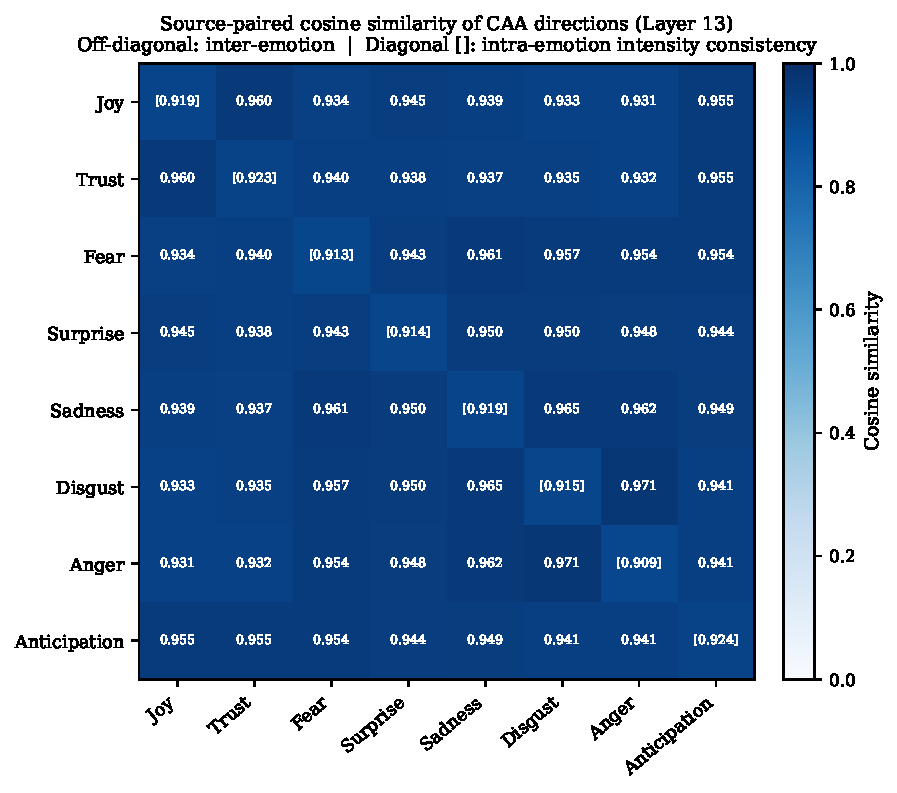
\includegraphics[width=0.75\linewidth]{figures/caa_paired_inter_emotion_cosine_heatmap_L13.pdf}
  \caption{Source-paired cosine similarity of CAA directions at layer 13. Off-diagonal: mean per-source cosine between emotion pairs. Diagonal \texttt{[\,]}: within-emotion intensity consistency (mean per-source cosine across low/medium/high intensity pairs). Colour scale spans $[0, 1]$; all entries lie above $0.90$.}
  \label{fig:caa_paired_inter_emotion_cosine_heatmap_L13}
\end{figure}

All values lie in the range $0.91$--$0.97$. More strikingly, for several emotion pairs such as \textit{disgust}--\textit{anger} ($0.971$) and \textit{sadness}--\textit{disgust} ($0.965$), the inter-emotion similarity \textbf{exceeds} the within-emotion intensity consistency shown on the diagonal ($0.91$--$0.92$). This means that for the same source text, the shift toward \textit{disgust} is more similar to the shift toward \textit{anger} than the low-intensity \textit{disgust} shift is to the high-intensity \textit{disgust} shift.\par

This uniformity would be unexpected if each CAA vector primarily encoded emotion-specific information. Instead, it suggests that \textbf{all vectors are dominated by a shared emotionalisation component}. This common axis is activated regardless of the targeted emotion. \par

The model appears to shift representations in two stages. First, it shifts from a neutral sentence to a generic emotional sentence. Then, from that shared emotional context, it moves towards a particular affective category. A raw CAA vector conflates both stages. This makes the emotion-specific signal difficult to access directly. This observation motivates the explicit decomposition introduced in the next section.\par

\section{Decomposition}
\label{sec:decomposition}

The pooled CAA vectors at layer 13 are highly aligned across emotion categories, suggesting that each vector contains a large shared component corresponding to generic emotionalisation. To separate this common shift from emotion identity, we define a shared vector as the normalised mean over emotion-specific pooled CAA vectors:
\[
\mathbf{g}=
\frac{\frac{1}{|E|}\sum_{e\in E}\mathbf{c}^{\mathrm{pool}}_{e,13}}
{\left\lVert\frac{1}{|E|}\sum_{e\in E}\mathbf{c}^{\mathrm{pool}}_{e,13}\right\rVert_2}.
\]
We then remove this shared component from each pooled vector by orthogonal projection:
\[
\mathbf{r}_e=\mathbf{c}^{\mathrm{pool}}_{e,13}-\left((\mathbf{c}^{\mathrm{pool}}_{e,13})^\top \mathbf{g}\right)\mathbf{g}.
\]
For steering, we use the unit-normalised residual
\[
\hat{\mathbf{r}}_e=\frac{\mathbf{r}_e}{\lVert\mathbf{r}_e\rVert_2},
\]
and construct interventions as
\[
\Delta_e(\alpha_G,\alpha_R)=\alpha_G\mathbf{g}+\alpha_R\hat{\mathbf{r}}_e.
\]

In this chapter, we treat this decomposition as an operational parameterisation for controllable steering: $\mathbf{g}$ controls global emotionalisation strength, while $\hat{\mathbf{r}}_e$ controls emotion-specific directionality. It is based on the same linear intervention assumption that underlies CAA. Behavioural features can be represented approximately as directions in the residual stream, and adding a vector in such a direction can modulate the corresponding behaviour causally. Assuming this, if emotion-specific CAA vectors are strongly aligned, their shared direction naturally estimates the component common to emotional responses across categories. \par

The mean direction, represented by the vector $\mathbf{g}$, captures the component that is consistently present across emotion categories. Since category-specific components are expected to vary with $e$, averaging over emotions should reduce idiosyncratic, identity-related components while preserving the common direction across all emotionalised generations. We therefore interpret $\mathbf{g}$ as an estimate of generic emotionalisation, i.e. a direction that increases the overall emotional character of the output independently of any particular emotion label. \par

The residual vector \(\mathbf{r}_e\) is obtained by subtracting the orthogonal projection of \(\mathbf{c}^{\mathrm{pool}}_{e,13}\) onto \(\mathbf{g}\), which removes the part of the emotion-specific CAA vector explained by the shared emotionalisation direction. Consequently, \(\mathbf{r}_e\) satisfies \(\mathbf{r}_e^\top \mathbf{g}=0\), meaning that, to first order in the linear residual-stream approximation, changes along \(\hat{\mathbf{r}}_e\) do not directly change the generic emotionalisation coordinate. The residual therefore isolates the remaining category-specific variation: the part of the vector that distinguishes one emotion from the shared emotional shift. \par

Further unit-normalising \(\mathbf{r}_e\) separates direction from intervention strength. The residual norm may depend on the size of the dataset, the variance within categories, the pooling choices made, or the strength with which a particular emotion is represented at layer 13. Using the normalised residual vector, the coefficient \(\alpha_R\) has a comparable interpretation across emotions: it controls how far the activation is moved in the category-specific residual direction rather than inheriting arbitrary differences in residual vector magnitude.\par

The final intervention
\[
\Delta_e(\alpha_G,\alpha_R)=\alpha_G\mathbf{g}+\alpha_R\hat{\mathbf{r}}_e
\]
therefore provides two independently interpretable steering controls. The coefficient \(\alpha_G\) modulates the shared emotionalisation component, while \(\alpha_R\) modulates the emotion-specific residual component. This makes it possible to test whether emotional intensity and emotion identity can be controlled separately: increasing \(\alpha_G\) should primarily increase the degree of emotionalisation, whereas increasing \(\alpha_R\) should primarily increase the recognisability of the target emotion.\par

This procedure should not be understood as recovering a single, accurate decomposition of emotional representations. Rather, it is a deliberately constrained linear decomposition, driven by the high degree of alignment observed among pooled emotion CAA vectors. The resulting two-parameter interventions are assessed for their empirical validity based on whether they exhibit the intended behavioural dissociation between generic emotionalisation and emotion-specific identity.\par

\begin{figure}[H]
    \centering
    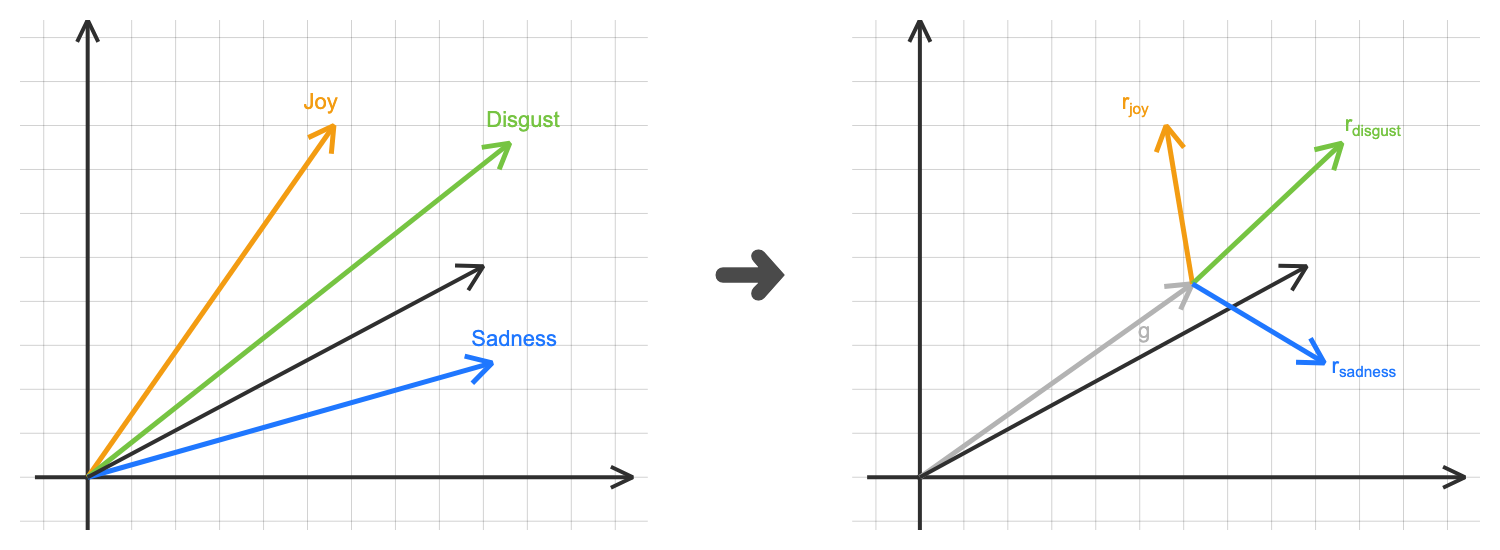
\includegraphics[width=0.8\linewidth]{figures/g_residualisation.png}
    \caption{Operational decomposition of emotion CAA vectors into a shared emotionalisation component $g$ and an emotion-specific residual component $\hat{r}_e$. The left panel shows the original CAA vectors for three example emotions (joy, disgust and sadness). The right panel shows the same vectors after removing the shared component $g$, revealing the residual vectors $\hat{r}_e$ that are specific to each emotion.}
    \label{fig:g_residualisation}
\end{figure}

\section{Decomposition Validity}
\label{sec:decomposition_validity}
%TODO

\section{Steering Experiments}
\label{sec:steering_experiments}

\subsection{Generation Setup}

We investigate whether emotion-specific residuals $\hat{\mathbf{r}}_e$ causally bias text generation towards the target emotion, and specifically, whether incorporating the shared vector $\mathbf{g}$ at any scale yields further benefits. We generate follow-up sentences using \texttt{Llama-3.1-8B-Instruct} from 100 source utterances sampled from the test split of the emotion rewriting dataset. To eliminate sampling variance as a confounding factor, we employ greedy decoding (temperature $= 0$) throughout the entire process.

\subsubsection*{Sweep Design}

Based on preliminary exploration, we fix $\alpha_R = 5.0$ as the residual scale that demonstrated the best performance, and scan $\alpha_G \in \{0, 0.25, 0.5, 1, 2, 3\}$. The anchor condition $\alpha_G = 0$ corresponds to pure residual steering (i.e. no shared components). The introduction of fine intermediate values ($0.25$, $0.5$, $1$, $2$) was intended to verify whether contributions from $\mathbf{g}$ below a certain threshold are beneficial before the scaling becomes detrimental. Each combination of source text, target emotion, and $\alpha_G$ value constitutes a single generation, resulting in a total of $100 \times 8 \times 6 = 4,800$ generated texts.


\subsection{Automated Evaluation Protocol}

Each generated sentence is scored by \texttt{gpt-4o-mini}, which acts as a judge. To ensure consistent evaluation criteria across all $4800$ items, the judge is presented with three fixed few-shot examples that cover the entire scoring range. Specifically, these are examples that match a high-quality target, examples where the meaning is preserved but the emotion expressed is incorrect, and examples where the target emotion is partially present but the propositional content is off-target. These examples serve to anchor the two endpoints of the evaluation scale before the evaluator views the test items. Scores are retrieved via OpenAI's Structured Output API, which utilises a strict JSON schema. This eliminates the need for free-form parsing and ensures that the three numerical scores and the dominant sentiment label are always returned in a consistent, machine-readable format. The evaluators operate without being informed of the intervention condition (the $\alpha_G$ value).

Three continuous $[0,1]$ metrics are collected per item:

\begin{itemize}
  \item \textbf{Target-emotion match}: Whether the predominant emotional tone of the output matches the target emotion. The judge is shown the target emotion label and asked to rate the degree to which the generated text conveys that emotion as its primary sentiment.
  \item \textbf{Semantic preservation}: Whether the core propositional content of the source utterance is retained. The judge compares the generated text with the original to assess whether the same events, entities, and relationships are present.
  \item \textbf{Emotionality}: Whether the output contains any emotional expression at all. A low score flags outputs that are flat, incoherent, or affectively empty, serving as a quality check: an intervention that appears to improve target-emotion match by producing incoherent text will be exposed by a corresponding drop on this metric.
\end{itemize}

\subsection{Statistical Analysis}

The mean values for each condition are reported together with the 95\% confidence intervals calculated from the score distributions for each item. To verify whether an arbitrary $\alpha_G > 0$ reliably exceeds the anchor value of $\alpha_G = 0$, items are paired using the key $({\rm source\_id},\,{\rm target\_emotion})$ for target emotion agreement, and a paired $t$-test is applied. By performing the pairing within this key, we control for sentence-level and emotion-level variations common to all $\alpha_G$ conditions, obtaining $n = 800$ pairs per test whilst achieving confidence intervals that are significantly narrower than those obtained in non-paired comparisons.

\subsection{Results}
\label{sec:alpha_g_sweep}

We hold $\alpha_R = 5.0$ fixed and sweep $\alpha_G \in \{0, 0.25, 0.5, 1, 2, 3\}$ across $n = 800$ samples per condition ($100$ source texts $\times$ $8$ target emotions). This directly answers whether adding $\mathbf{g}$ helps at any scale.

Figure~\ref{fig:alpha_g_sweep_aggregate} shows all three metrics as a function of $\alpha_G$. All three decline monotonically as $\alpha_G$ increases. Target-emotion match falls from $0.270$ at $\alpha_G = 0$ to $0.252$ at $\alpha_G = 3$; emotionality drops from $0.567$ to $0.531$; and semantic preservation declines from $0.870$ to $0.863$. No value of $\alpha_G > 0$ produces any reliable improvement over $\alpha_G = 0$ on any metric. The per-emotion breakdown (Figure~\ref{fig:alpha_g_sweep_per_emotion}) confirms that no individual emotion benefits from a positive $\alpha_G$.

\begin{figure}[H]
\centering
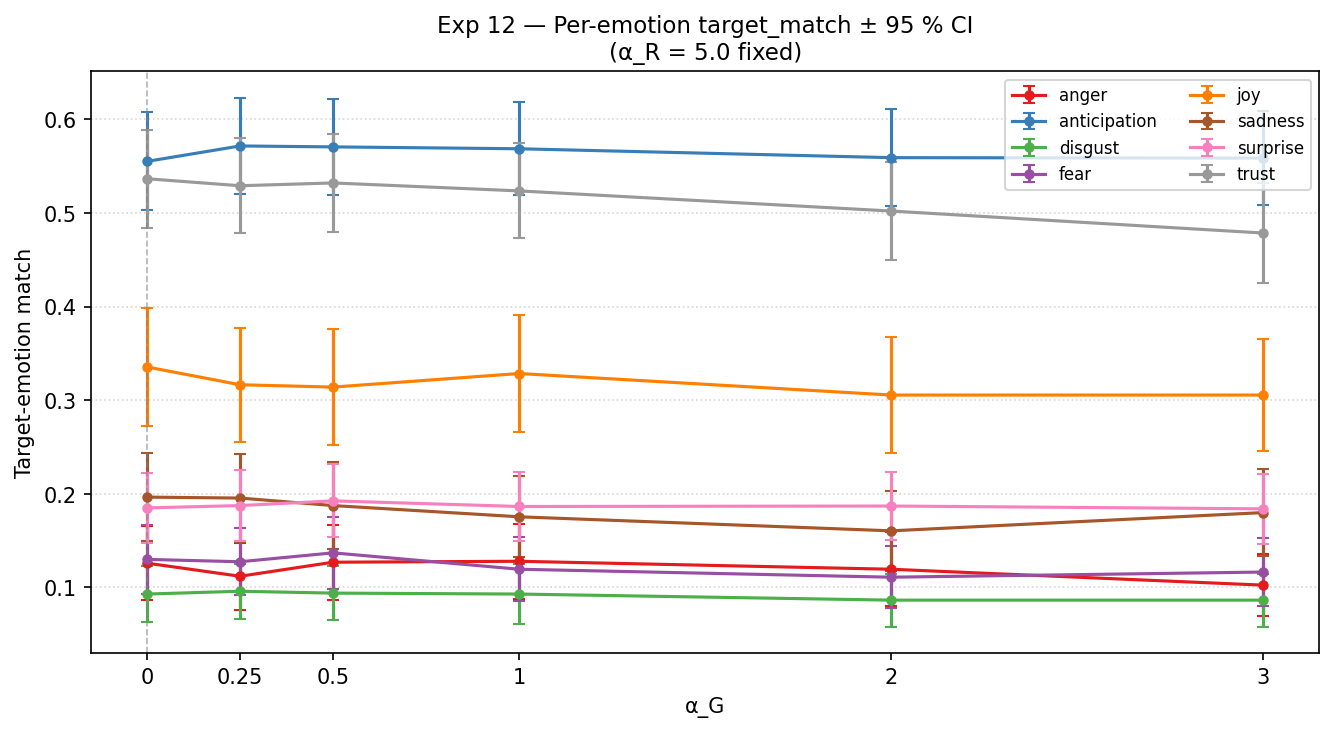
\includegraphics[width=\linewidth]{figures/alpha_g_sweep_per_emotion.png}
\caption{Per-emotion target-emotion match vs.\ $\alpha_G$ ($\alpha_R = 5.0$ fixed; $n = 100$ per cell; error bars = 95\% CI). No individual emotion benefits from a positive $\alpha_G$.}\label{fig:alpha_g_sweep_per_emotion}
\end{figure}

\begin{figure}[H]
\centering
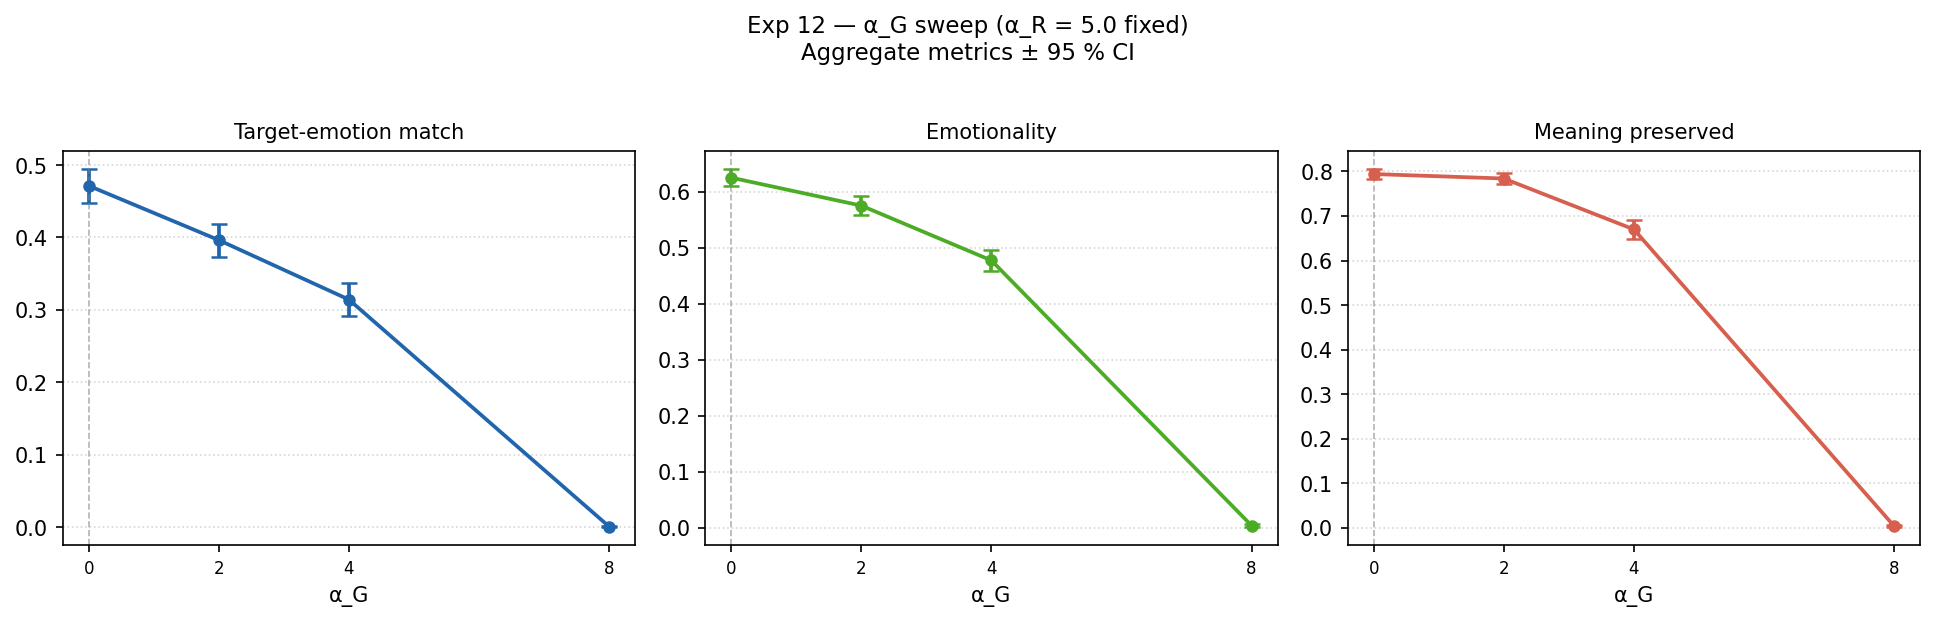
\includegraphics[width=\linewidth]{figures/alpha_g_sweep_aggregate.png}
\caption{Target-emotion match, emotionality, and semantic preservation as a function of $\alpha_G$, with $\alpha_R = 5.0$ fixed ($n = 800$ per condition; error bars = 95\% CI). All three metrics decrease monotonically as $\alpha_G$ increases from $0$.}\label{fig:alpha_g_sweep_aggregate}
\end{figure}

The shared direction $\mathbf{g}$ is counterproductive at every tested scale. Effective affective steering therefore reduces to $\Delta_e = \alpha_R\,\hat{\mathbf{r}}_e$, with $\alpha_G$ discarded.

\section{Causal Validation: Steering}
\label{sec:steering_causal_validation}

To confirm that the emotion-specific residual $\hat{\mathbf{r}}_e$ provides a reliable steering signal, we perform a generation experiment using pure residual steering ($\alpha_G = 0$, $\alpha_R = 5.0$). This tests whether adding $\hat{\mathbf{r}}_e$ alone can bias generation towards the target emotion, and whether the resulting outputs exhibit the expected pattern of emotional shift without excessive loss of semantic content.

\subsection{Activation Hook}
The steering intervention is implemented as a forward hook registered in the layer 13 of the transformer. In each forward pass, this hook captures the hidden state $\mathbf{h} \in \mathbb{R}^{B \times T \times D}$ of the residual stream generated by that layer, and adds $\Delta_e$ only to the slice of the final token:
\[
\mathbf{h}_{:,\,-1,\,:} \;\leftarrow\; \mathbf{h}_{:,\,-1,\,:} + \Delta_e(\alpha_G, \alpha_R),
\]
where $\Delta_e = \alpha_G\,\mathbf{g} + \alpha_R\,\hat{\mathbf{r}}_e$. By applying the perturbation only to the final prompt token, we concentrate the causal signal at the point where the model begins its autoregressive generation, whilst keeping the contextual representations of all preceding tokens unchanged. To prevent interference between invocations, the hook is released immediately after generation is complete.

\subsection{Result}

Table~\ref{tab:qualitative_steering_examples} shows representative examples of residual-only steering ($\alpha_G = 0$, $\alpha_R = 5$, last-token intervention at layer 13). The intervention does not simply overwrite the source context; instead, it bends the existing situation toward the target affective framing.

\begin{table}[H]
\centering
\small
\begin{tabular}{p{0.13\linewidth} p{0.13\linewidth} p{0.30\linewidth} p{0.34\linewidth}}
\toprule
\textbf{Seed} & \textbf{Target} & \textbf{Seed utterance} & \textbf{Steered output} \\
\midrule
fear & joy &
Walking alone through the dark alley I felt a cold shiver run down my spine. &
As I strolled through the dimly lit alley, the flickering streetlights cast a warm glow, but the sense of solitude and tranquility that filled the air made me feel a gentle, soothing calm wash over me. \\
\midrule
disgust & joy &
The smell from the bin was overwhelming and the sight of it made my stomach turn. &
The putrid aroma wafting from the trash can was a welcome respite, and the vibrant colors of the discarded items made my heart feel uplifted. \\
\bottomrule
\end{tabular}
\caption{Representative examples of residual-only CAA steering ($\alpha_G = 0$, $\alpha_R = 5$). The fear-to-joy example shows a natural affective shift while preserving the dark-alley context. The disgust-to-joy example shows a more extreme reinterpretation, illustrating both the causal reach and the contextual limits of the intervention.}
\label{tab:qualitative_steering_examples}
\end{table}

Both examples illustrate the same pattern: the residual intervention shifts the emotional framing without replacing the underlying situation. The fear-to-joy output preserves the alley but reframes it as tranquil; the disgust-to-joy output retains the bin but reinterprets its contents positively. The final output remains bounded by the semantic content of the source, consistent with the modest but consistent target-emotion match gains seen in the quantitative results.

\subsection{Interpretation}

The $\alpha_G$ sweep gives a clear answer: adding the shared emotionalisation direction $\mathbf{g}$ hurts performance at every tested scale. All three evaluation metrics decline monotonically as $\alpha_G$ increases, and this holds for all eight target emotions without exception. The practical conclusion is that the two-component formula $\Delta_e = \alpha_G\,\mathbf{g} + \alpha_R\,\hat{\mathbf{r}}_e$ reduces in practice to its residual term alone: $\Delta_e = \alpha_R\,\hat{\mathbf{r}}_e$.\par

This finding also clarifies what the decomposition achieves. The pooled CAA vector $\mathbf{c}^{\mathrm{pool}}_e$ is dominated by $\mathbf{g}$ (as the high cross-emotion cosine similarities in Section~\ref{sec:caa_construction} showed), so steering with the raw pooled vector is largely equivalent to adding $\mathbf{g}$~--and therefore counterproductive. The decomposition separates $\mathbf{g}$ from $\hat{\mathbf{r}}_e$ precisely so that the useful component can be used in isolation. The steering effect is modest rather than absolute: the intervention biases the output toward the target emotion while remaining constrained by the initial utterance, and larger $\alpha_R$ provides only partial directional control. These limitations motivate the structural analysis of $\hat{\mathbf{r}}_e$ in the next chapter.\par

\section{Limitations and Transition}

These results confirm that affective steering can be implemented as a decomposed residual-space intervention, and that the effective operating point is $\alpha_G = 0$, $\alpha_R > 0$. The shared direction $\mathbf{g}$ is counterproductive at every tested scale; only the emotion-specific residual $\hat{\mathbf{r}}_e$ provides a reliable steering signal. This conclusion was only reachable because the decomposition made the two components separable and independently testable.\par

However, the results also reveal two limitations. First, the steering effect is modest rather than absolute: target-emotion match improves consistently but remains well below ceiling, and the intervention is bounded by the semantic and emotional content of the source utterance. Second, the effect magnitude varies substantially across emotions, suggesting that the discriminative power of $\hat{\mathbf{r}}_e$ differs by emotion category — a structural question addressed in the next chapter.\par

These limitations motivate the next chapter. So far, $\hat{\mathbf{r}}_e$ has been treated as a single entity. The next chapter asks what this residual actually represents. In particular, it examines whether emotions such as joy, sadness, and anger should be treated as atomic vectors, or whether they contain local sub-axes that correspond to more subtle, pre-verbal affective vectors.
\chapter{Pre-Verbal Affective Vector Projection}

The previous chapter established that, for a given target emotion $e$, the decomposed steering vector
\[
\Delta_e(\alpha_G,\alpha_R)=\alpha_G\mathbf{g}+\alpha_R\hat{\mathbf{r}}_e
\]
reliably shifts the affective framing of generated text towards $e$ while preserving semantic content.
In that framework, joy, sadness, anger, and the other Plutchik categories were treated as
\emph{primitive} units: each $\hat{\mathbf{r}}_e$ was taken to be an irreducible
emotion-specific direction without further decomposition.

This chapter re-examines that assumption.
The central question is whether named emotion categories such as \emph{joy} or \emph{fear}
are the minimal units of affective representation in the model's residual stream,
or whether each $\hat{\mathbf{r}}_e$ is itself a composite, structured along a small set of
more fundamental, pre-categorical affective dimensions.
The experiments reported here provide evidence for the latter: within each named emotion there
exist local sub-axes, these sub-axes are largely shared across emotion categories, and they can be
interpreted as dimensions that are more primitive than any named emotion label.
The central conclusion is that what Chapter~1 called $\hat{\mathbf{r}}_e$
can be re-read as a projection onto a shared pre-verbal affective space:
\[
\hat{\mathbf{r}}_e
\;=\;
\sum_{k=1}^{K}\beta_{e,k}\,\mathbf{m}_k
\;+\;
\boldsymbol{\varepsilon}_e,
\]
where $\mathbf{m}_k$ are label-free meta-axes shared across all emotions,
$\beta_{e,k}=\hat{\mathbf{r}}_e^\top\mathbf{m}_k$ are scalar projections that encode the
``affective fingerprint'' of emotion $e$, and $\boldsymbol{\varepsilon}_e$ is the residual
component that is orthogonal to all $\mathbf{m}_k$.

\section*{Experimental Roadmap}

This chapter is organised as follows.
\begin{enumerate}
  \item \textbf{Discriminability of $\hat{\mathbf{r}}_e$}: We first verify that the residual
    $\hat{\mathbf{r}}_e$ is a genuine emotion-specific signal rather than noise, motivating the
    search for its internal structure.
  \item \textbf{Internal variance structure}: We characterise the internal dimensionality of
    each named emotion by applying PCA to the distribution of per-source residual vectors
    within each emotion category.
  \item \textbf{Local sub-axis extraction and interpretation}: We extract the leading
    principal directions within each emotion and submit them to an LLM judge for semantic
    interpretation. We also confirm that these axes are affective rather than stylistic
    artefacts.
  \item \textbf{Cross-emotion sharing}: We show that the local PCA axes cluster by
    \emph{rank} rather than by emotion label, revealing a set of shared meta-axes
    $\mathbf{m}_k$ that span all named emotions.
  \item \textbf{Extraction and formalisation of meta-axes}: We formalise $\mathbf{m}_k$ as
    sign-aligned means over per-emotion PCA directions, and assess their stability.
  \item \textbf{Pre-verbal interpretation}: We interpret each $\mathbf{m}_k$ by presenting
    extreme examples from \emph{all} emotions simultaneously to an LLM judge, obtaining
    emotion-independent semantic labels for each meta-axis.
  \item \textbf{Re-decomposition of $\hat{\mathbf{r}}_e$}: We project each $\hat{\mathbf{r}}_e$
    onto the $\mathbf{m}_k$ basis, quantify the explained variance, and state the
    revised decomposition that extends the formula from Chapter~1.
  \item \textbf{Causal validation -- local axis steering}: We test whether adding
    $\pm\beta\,\mathbf{u}_{e,1}$ or $\pm\beta\,\mathbf{m}_1$ to the steering vector causally
    shifts outputs along the expected affective sub-dimension.
  \item \textbf{Label-free steering}: We compare three steering conditions---named emotion
    prototype only, $\mathbf{m}_k$-projection only, and their combination---to determine
    whether the $\mathbf{m}_k$ decomposition retains the practical utility of $\hat{\mathbf{r}}_e$.
\end{enumerate}

% ─────────────────────────────────────────────────────────────
\section{Geometric Overview of the Affective Residual Space}
\label{sec:ch2-geometry}

Before asking whether $\hat{\mathbf{r}}_e$ has internal sub-structure, we characterise the
geometry of the eight emotion-specific directions as a whole.
This provides a baseline picture of what kind of space $\hat{\mathbf{r}}_e$ lives in, and
motivates the specific questions that follow.

\subsection*{Raw directions are near-collinear}

At layer~13, the pairwise cosine similarities among the eight pooled CAA directions
$\mathbf{c}^{\mathrm{pool}}_e$ are extremely high.
The mean off-diagonal cosine is $0.986$, and even Plutchik opposite pairs
(e.g., joy--sadness, trust--disgust) have a mean cosine of $0.984$, nearly indistinguishable
from adjacent pairs ($0.988$).
This near-collinearity is the signature of the dominant shared component $\mathbf{g}$:
all eight directions point in almost the same direction because the largest component of
any emotional activation is simply the shift from neutral to emotional.

Despite this, PCA over the eight pooled directions reveals a low-dimensional but
non-trivial structure: the participation ratio is $3.61$, with
$\mathrm{EVR}_{\mathrm{PC1}}=0.437$ and $\mathrm{EVR}_{\mathrm{PC1\text{-}3}}=0.812$.
Even before any explicit decomposition, emotion directions do not fill eight independent
dimensions; they are organised within roughly three to four effective axes.

\subsection*{Residualisation exposes structured negative geometry}

After removing $\mathbf{g}$, the geometry changes qualitatively.
The residual directions $\mathbf{r}_e = \mathbf{c}_e - (\mathbf{c}_e^\top\mathbf{g})\mathbf{g}$
have a mean off-diagonal cosine of $-0.137$.
Plutchik opposite pairs become clearly negative on average ($-0.306$), while adjacent pairs
remain weakly positive ($+0.090$).
This sign reversal shows that the residual space encodes emotion-specific structure that
is consistent with Plutchik's theoretical organisation of emotions.

\begin{figure}[H]
  \centering
  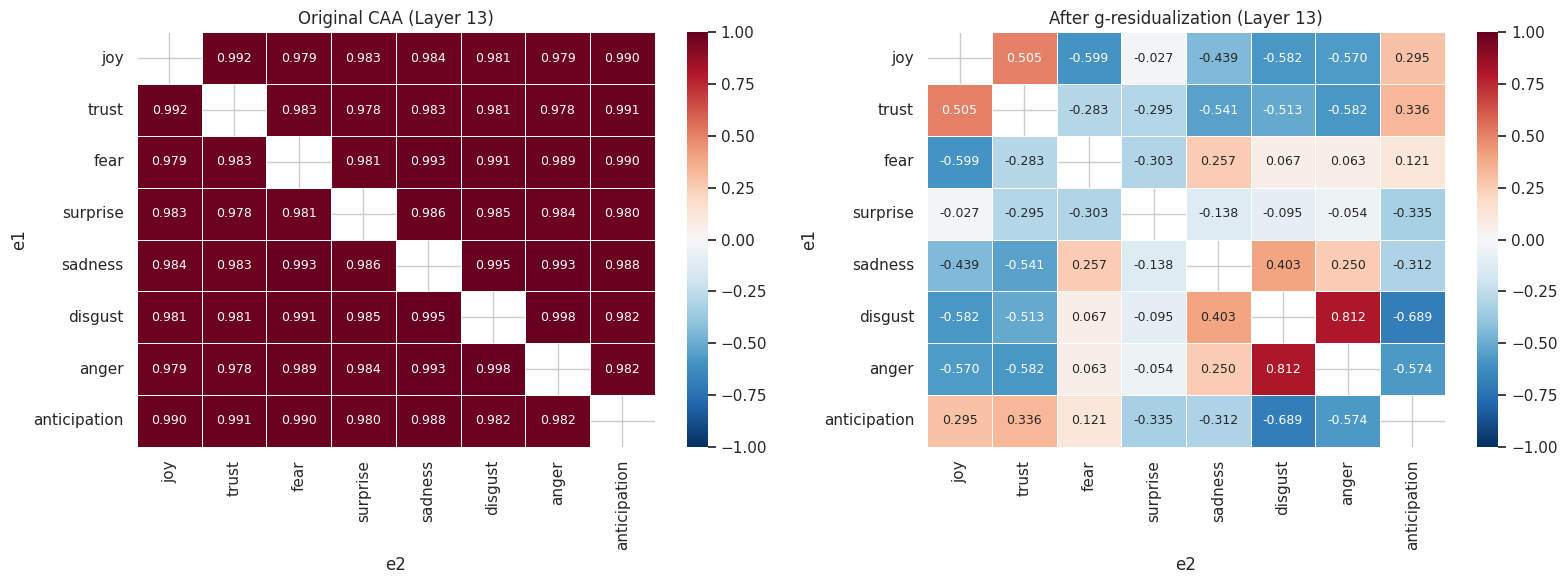
\includegraphics[width=0.80\linewidth]{figures/cosine_heatmap_before_after_L13.png}
  \caption{Pairwise cosine similarities among pooled CAA directions before (left) and
           after (right) removal of the shared emotionalisation component $\mathbf{g}$
           at layer~13. Before residualisation, all directions are near-collinear.
           After residualisation, Plutchik opposite pairs become negative and the
           emotion-specific structure is revealed.}
  \label{fig:cosine_before_after}
\end{figure}

\begin{figure}[H]
  \centering
  
\includegraphics[width=0.80\linewidth]{figures/plutchik_pairs_before_after.png}
  \caption{Mean cosine similarity of Plutchik opposite and adjacent emotion pairs
           across layers, before and after $\mathbf{g}$-residualisation.
           The crossover of opposite-pair cosines from positive to negative after
           residualisation is consistent across candidate layers.}
  \label{fig:plutchik_pairs}
\end{figure}

\subsection*{Residual directions are low-dimensional but internally heterogeneous}

Importantly, the residual space remains low-dimensional after this operation:
the participation ratio changes only from $3.61$ to $3.63$, and
$\mathrm{EVR}_{\mathrm{PC1}}=0.448$ for the eight $\mathbf{r}_e$ centroids.
This indicates that the emotion-specific information is not scattered across a
high-dimensional space but is organised within roughly four effective dimensions.

At the same time, per-source analysis reveals that the individual delta vectors
$\boldsymbol{\delta}_{n,e}$ within each named emotion are not tightly concentrated around their
centroid $\mathbf{r}_e$.
Local PCA within each emotion yields participation ratios of approximately $3.5$--$3.7$
(for the top-5 component analysis), and the first local PC accounts for only $11$--$12\%$
of intra-emotion variance.
In other words, while $\mathbf{r}_e$ is a good summary direction for emotion $e$, each
emotion behaves more like a \emph{cone} or a \emph{prototype region} with internal
sub-axes than like a single, thin direction.

\subsection*{The implication: r̂_e has internal structure worth investigating}

Together, these observations motivate the core question of this chapter.
The residual directions $\hat{\mathbf{r}}_e$ are meaningful (Plutchik geometry is
preserved), structured (low-dimensional), but internally heterogeneous (each emotion
spans a cone rather than a point).
The experiments that follow ask: what are the axes within each cone, are they shared
across emotions, and do they correspond to interpretable pre-verbal affective dimensions?

% ─────────────────────────────────────────────────────────────
\section{Discriminability of the Emotion-Specific Residual}
\label{sec:ch2-discriminability}

% Exp1: after removing g, r_e still decodes emotion labels at ~85% balanced accuracy.
% This section answers: is r_e meaningful beyond the emotionalisation component?

Before asking about the internal geometry of $\hat{\mathbf{r}}_e$, we first confirm that it
carries genuine emotion-specific information.
If $\hat{\mathbf{r}}_e$ were merely the small orthogonal complement of a dominant
emotionalisation direction and contained no structured signal, the internal analysis that
follows would be unmotivated.

\subsection*{Protocol}

For each source utterance $n$ and emotion $e$, we define the per-source affective shift
\[
\boldsymbol{\delta}_{n,e}
=\mathbf{h}^{\mathrm{emo}}_{n,e}-\mathbf{h}^{\mathrm{neu}}_{n},
\]
and remove the shared emotionalisation direction $\mathbf{g}$:
\[
\boldsymbol{\delta}^{g\perp}_{n,e}
=\boldsymbol{\delta}_{n,e}-(\boldsymbol{\delta}_{n,e}^\top\mathbf{g})\mathbf{g}.
\]
We then train a linear probe (PCA-64 $\to$ standardised logistic regression) to predict the
emotion label $e$ from $\boldsymbol{\delta}^{g\perp}_{n,e}$, using five-fold cross-validation
grouped by source identity to prevent leakage.
Chance level is $1/8=0.125$.

\subsection*{Results}

% Table: balanced accuracy by layer (from exp1)
\begin{table}[H]
\centering
\small
\begin{tabular}{lcc}
\toprule
\textbf{Layer} & \textbf{Balanced accuracy} & \textbf{Std} \\
\midrule
10 & 0.853 & 0.002 \\
13 \textbf{*} & \textbf{0.857} & 0.001 \\
16 & 0.755 & 0.002 \\
\bottomrule
\end{tabular}
\caption{Emotion-label balanced accuracy from a linear probe trained on
         $\boldsymbol{\delta}^{g\perp}_{n,e}$ (affective shift with shared emotionalisation
         removed). Asterisk marks the primary reporting layer selected in Chapter~1.
         Chance level is $0.125$.}
\label{tab:exp1_probe_accuracy}
\end{table}

At layer~13, balanced accuracy reaches $0.857$, nearly seven times the chance level.
This demonstrates that the g-residualised shifts contain strong, linearly decodable
emotion-category information independent of the shared emotionalisation component.
The signal peaks at layers~10--13 and decays monotonically at deeper layers, consistent with
a representation that is transformed from qualitative affective identity towards
next-token prediction at higher depths.

\subsection*{Interpretation}

The high discriminability of $\boldsymbol{\delta}^{g\perp}_{n,e}$ confirms that
$\hat{\mathbf{r}}_e$ is not noise.
It encodes the qualitative difference between \emph{joy}, \emph{sadness}, \emph{anger}, and
so on.
This motivates the next question: what is the internal geometric structure of these directions?

% ─────────────────────────────────────────────────────────────
\section{Internal Variance Structure of Named Emotions}
\label{sec:ch2-variance-structure}

% Exp2: per-emotion PCA, participation ratio analysis.
% joy/trust concentrated; fear/surprise diffuse.
% Named emotions differ in their internal dimensionality.

The previous section shows that $\hat{\mathbf{r}}_e$ is a genuine signal.
A single vector, however, summarises an entire distribution: for each emotion $e$, there are
$N \times I$ per-source residual vectors $\boldsymbol{\delta}^{g\perp}_{n,e,i}$, and $\hat{\mathbf{r}}_e$
is their normalised average.
This section asks whether the \emph{distribution} is concentrated around a single
direction or whether it spans multiple dimensions.

\subsection*{Protocol}

For each emotion $e$, we collect the per-source, per-intensity residuals
$\boldsymbol{\delta}^{g\perp}_{n,e,i}$ at layer~13, apply PCA, and compute the participation
ratio
\[
\mathrm{PR}_e
=\frac{\left(\sum_k \lambda_k\right)^2}{\sum_k \lambda_k^2},
\]
where $\lambda_k$ are the eigenvalues of the empirical covariance.
To establish a baseline, we shuffle the emotion labels to destroy emotion-specific structure
and report $\mathrm{PR}_{\mathrm{shuffle}}$.
A value $\mathrm{PR}_e < \mathrm{PR}_{\mathrm{shuffle}}$ indicates that the emotion's
internal distribution is \emph{more concentrated} than random, whereas
$\mathrm{PR}_e > \mathrm{PR}_{\mathrm{shuffle}}$ indicates a \emph{more diffuse}, multi-axis
structure.

\subsection*{Results}

% Table: participation ratio (from exp2)
\begin{table}[H]
\centering
\small
\begin{tabular}{lccc}
\toprule
\textbf{Emotion} & \textbf{PR} & \textbf{PR (shuffle)} & \textbf{PR excess} \\
\midrule
joy        &  6.72 & 13.62 & $-6.90$ \\
trust      & 10.54 & 13.65 & $-3.11$ \\
sadness    & 12.11 & 13.59 & $-1.48$ \\
disgust    & 12.74 & 13.61 & $-0.87$ \\
anticipation & 15.30 & 13.65 & $+1.65$ \\
anger      & 15.56 & 13.63 & $+1.93$ \\
fear       & 18.16 & 13.60 & $+4.57$ \\
surprise   & 18.94 & 13.63 & $+5.31$ \\
\bottomrule
\end{tabular}
\caption{Participation ratio of per-source affective shift distributions at layer~13.
         A negative excess indicates a concentrated, near-uniaxial structure;
         a positive excess indicates a diffuse, multi-axis structure.}
\label{tab:exp2_participation_ratio}
\end{table}

The results reveal a clear gradient: joy and trust have highly concentrated
internal distributions (PR well below shuffle), whereas fear and surprise are substantially
more diffuse (PR well above shuffle).
Named emotions are therefore not equivalent in their internal dimensionality: some are
almost prototype-like, while others occupy broader affective regions.

\subsection*{Interpretation}

Each named emotion category is not a single, thin direction but a cone or region with
its own internal geometry.
The variation across the $N \times I$ per-source residuals encodes sub-distinctions
within joy, within fear, and so on.
This internal structure is the subject of the next section.

% ─────────────────────────────────────────────────────────────
\section{Local Sub-Axes and Their Affective Interpretation}
\label{sec:ch2-local-axes}

% Exp3 + Exp4: PCA within each emotion's residuals → local sub-axes u_{e,k}.
% LLM judge interpretations. Style contamination check.

The participation ratio analysis shows that each named emotion has non-trivial internal
variation.
We now characterise this variation explicitly by extracting local principal axes.

\subsection*{Extraction pipeline}
\label{subsec:local-axis-pipeline}

Starting from the per-source affective shifts, we apply the following residualisation steps
before extracting emotion-internal principal components.

\begin{enumerate}
  \item Compute the base shift:
    $\boldsymbol{\delta}_{n,e,i} = \mathbf{h}^{\mathrm{emo}}_{n,e,i} - \mathbf{h}^{\mathrm{neu}}_{n}$.
  \item Remove the shared emotionalisation direction:
    $\boldsymbol{\delta}^{(1)}_{n,e,i} = \boldsymbol{\delta}_{n,e,i} - (\boldsymbol{\delta}_{n,e,i}^\top\mathbf{g})\mathbf{g}$.
  \item Remove the per-emotion intensity direction $\mathbf{u}_e$
    (the normalised mean of $\boldsymbol{\delta}^{(1)}_{n,e,\cdot}$ over intensities $i$):
    $\boldsymbol{\delta}^{(2)}_{n,e,i} = \boldsymbol{\delta}^{(1)}_{n,e,i} - (\boldsymbol{\delta}^{(1)}_{n,e,i}{}^\top\mathbf{u}_e)\mathbf{u}_e$.
  \item Remove source-wise mean (mean over emotions for the same source $n$):
    $\boldsymbol{\delta}^{(3)}_{n,e,i} = \boldsymbol{\delta}^{(2)}_{n,e,i} - \frac{1}{|E|}\sum_{e'}\boldsymbol{\delta}^{(2)}_{n,e',i}$.
\end{enumerate}

For each emotion $e$, we collect the matrix
$\{\boldsymbol{\delta}^{(3)}_{n,e,i}\}_{n,i}$ and apply PCA.
The $k$-th principal component is denoted $\mathbf{u}_{e,k}$; it is the direction of maximal
residual variance within emotion $e$ that is orthogonal to $\mathbf{g}$ and to $\mathbf{u}_e$.

\subsection*{Interpretation of local sub-axes}

We submit the top-5 and bottom-5 example texts for each $\mathbf{u}_{e,k}$ to an
LLM judge (GPT-4o) and ask it to label the axis semantically.
Table~\ref{tab:local_axis_pc1} summarises the leading axis for each emotion,
along with judge-assigned contamination and confidence scores.

% Table: PC1 interpretations (from exp3)
\begin{table}[H]
\centering
\small
\begin{tabular}{p{0.15\linewidth} p{0.47\linewidth} p{0.12\linewidth} p{0.12\linewidth}}
\toprule
\textbf{Emotion} & \textbf{PC1 axis name} & \textbf{Contam.} & \textbf{Conf.} \\
\midrule
joy          & Reflective/perspective-taking joy \emph{vs} immediate/external event joy       & medium & 4 \\
trust        & Trust as hopeful acceptance \emph{vs} self-assured confidence                   & medium & 5 \\
fear         & Immediate situational anxiety \emph{vs} chronic/existential worry               & low    & 5 \\
surprise     & Unexpected events \emph{vs} expected/anticipated events                         & low    & 5 \\
sadness      & Loss \& disappointment \emph{vs} everyday contentment                           & low    & 5 \\
disgust      & Visceral sensory repulsion \emph{vs} mild/abstract discomfort                   & medium & 4 \\
anger        & Irritation/frustration \emph{vs} disappointment/resigned upset                  & low    & 5 \\
anticipation & Hopeful curiosity \emph{vs} uneasy waiting                                      & low    & 5 \\
\bottomrule
\end{tabular}
\caption{LLM-judge interpretations of the leading local sub-axis $\mathbf{u}_{e,1}$ for each
         emotion at layer~13.
         Five of eight emotions achieve contamination = low and confidence = 5, indicating
         that the extracted axes capture genuine affective distinctions rather than stylistic
         variation.}
\label{tab:local_axis_pc1}
\end{table}

\subsection*{Style contamination check}
\label{subsec:style-contamination}

% Exp4: 34/40 axes classified as likely_affective; Methods A/B/C.

To confirm that the local axes are affective rather than artefacts of text style or topic,
we apply three independent checks to all 40 axes (8 emotions $\times$ 5 PCs).

\begin{itemize}
  \item \textbf{Method A (style-feature probe).} We regress the PC scores on a battery of
    surface features (sentence length, lexical diversity, POS ratios, etc.).
    Mean $R^2$ over 40 axes is $0.069$; only 5 axes exceed the threshold of $0.15$.
  \item \textbf{Method B (neutral-control alignment).} We extract PCA axes from the neutral
    paraphrase activations and measure cosine alignment with each local PC.
    Mean maximum cosine is $0.034$, uniformly low, indicating no systematic confound from
    paraphrase-level style variation.
  \item \textbf{Method C (meaning-preservation filter).} We restrict the analysis to
    rewrites that pass a semantic-similarity filter and recompute PCA axes.
    Mean cosine between full and filtered axes is $0.944$; only 1 of 40 axes
    ($\mathrm{surprise}\text{ PC5}$) drops below the robustness threshold of $0.70$.
\end{itemize}

Based on these three checks, 34 of 40 axes are classified as \textbf{likely affective},
6 as ambiguous, and none as likely stylistic.
The local PCA axes therefore reflect genuine sub-distinctions within the affective content of
each emotion category rather than co-varying surface features.

% ─────────────────────────────────────────────────────────────
\section{Cross-Emotion Sharing: From Local Axes to Meta-Axes}
\label{sec:ch2-meta-axes}

% Exp6: clustering shows PC-rank, not emotion-label, determines similarity.
% Exp7: formalise m_k.

So far, the local sub-axes $\mathbf{u}_{e,k}$ have been characterised separately for each
emotion.
We now ask whether these axes are emotion-specific or whether they encode dimensions that
recur across emotions.
This turns out to be a crucial question: if the sub-axes are shared, then the internal
variation of each named emotion is organised along the same underlying dimensions,
and $\hat{\mathbf{r}}_e$ can be re-read as a specific pattern of activations along those
shared dimensions.

\subsection*{Clustering reveals PC-rank, not emotion label, as the organising principle}

% Exp6 main result
We compute the absolute cosine similarity between all 40 local PC vectors (8 emotions $\times$
5 PCs) and apply Ward hierarchical clustering.
The resulting dendrogram reveals a striking pattern: the dominant clusters group axes by
their \emph{rank} ($k=1,2,3$) rather than by emotion label.
Specifically:
\begin{itemize}
  \item The $k=1$ axes of all eight emotions form a single, tight cluster
    ($|\cos|\approx 0.74$--$0.95$ across all pairs).
  \item The $k=2$ axes of all eight emotions form a second cluster.
  \item The $k=3$ axes similarly form a third cluster.
  \item Emotion-specific structure first appears at $k=4$ and $k=5$.
\end{itemize}

This organisation is confirmed by cross-emotion cosine similarities at the PC1 level
(Table~\ref{tab:cross_emotion_cosine_pc1}) and by meta-PCA over the 40 vectors,
where the top-3 meta-components capture 51\% of the total variance across
all emotion-PC combinations and separate by rank.

\begin{table}[H]
\centering
\small
\begin{tabular}{lcc}
\toprule
\textbf{Emotion pair (PC1)} & $|\cos(\mathbf{u}_{e_1,1},\mathbf{u}_{e_2,1})|$ \\
\midrule
disgust -- anger    & 0.950 \\
sadness -- disgust  & 0.922 \\
trust   -- disgust  & 0.886 \\
joy     -- anger    & 0.874 \\
fear    -- disgust  & 0.839 \\
anticipation -- sadness & 0.805 \\
surprise -- sadness & 0.743 \\
\bottomrule
\end{tabular}
\caption{Cross-emotion absolute cosine similarity for the leading local sub-axis
         $\mathbf{u}_{e,1}$. All pairs are well above chance, indicating a universal
         primary axis shared across all eight named emotions.}
\label{tab:cross_emotion_cosine_pc1}
\end{table}

\subsection*{Formalisation of meta-axes $\mathbf{m}_k$}
\label{subsec:meta-axis-def}

% Exp7: sign-aligned mean, method agreement
Given that $k$-th rank local axes cluster tightly across emotions, we define a shared
\textbf{meta-axis} $\mathbf{m}_k$ as the normalised sign-aligned mean of the $k$-th local
PC vectors:
\[
\mathbf{m}_k
=\frac{\sum_{e\in E}\sigma_{e,k}\,\mathbf{u}_{e,k}}
      {\left\lVert\sum_{e\in E}\sigma_{e,k}\,\mathbf{u}_{e,k}\right\rVert_2},
\]
where $\sigma_{e,k}\in\{+1,-1\}$ is chosen by sign-aligning $\mathbf{u}_{e,k}$ with the
first emotion's axis so that all vectors point in a consistent direction before averaging.

As a robustness check, we also extract $\mathbf{m}_k$ via group PCA (applying PCA to the
sign-aligned set of $k$-th rank vectors) and measure the cosine between the two estimates.

\begin{table}[H]
\centering
\small
\begin{tabular}{lcc}
\toprule
\textbf{Meta-axis} & $|\cos(\mathbf{m}_k^{\mathrm{mean}},\mathbf{m}_k^{\mathrm{pca}})|$
  & \textbf{Mean $|\cos|$ to $\mathbf{u}_{e,k}$} \\
\midrule
$\mathbf{m}_1$ & 0.990 & 0.892 \\
$\mathbf{m}_2$ & 0.829 & 0.800 \\
$\mathbf{m}_3$ & 0.989 & 0.672 \\
$\mathbf{m}_4$ & 0.266 & 0.437 \\
$\mathbf{m}_5$ & 0.104 & 0.427 \\
\bottomrule
\end{tabular}
\caption{Stability of meta-axes $\mathbf{m}_k$. The first column reports agreement between
         the two extraction methods (sign-aligned mean vs.\ group PCA); the second reports
         mean absolute cosine between $\mathbf{m}_k$ and the individual local axes
         $\mathbf{u}_{e,k}$.
         Meta-axes $\mathbf{m}_1$--$\mathbf{m}_3$ are stable and representative;
         $\mathbf{m}_4$ and $\mathbf{m}_5$ are not.}
\label{tab:meta_axis_stability}
\end{table}

Meta-axes $\mathbf{m}_1$, $\mathbf{m}_2$, and $\mathbf{m}_3$ are stable under
method variation (method agreement $\geq 0.83$) and well-aligned with the individual local
axes (mean $|\cos| \geq 0.67$).
Meta-axes $\mathbf{m}_4$ and $\mathbf{m}_5$ show poor method agreement ($0.27$ and $0.10$)
and are excluded from further interpretation.

Two additional properties of the stable meta-axes are noteworthy.
First, all $\mathbf{m}_k$ are nearly orthogonal to the shared emotionalisation direction
$\mathbf{g}$ ($|\cos(\mathbf{m}_k,\mathbf{g})| < 0.02$ for all $k$), confirming that they
capture \emph{affective texture} rather than overall emotionalisation strength.
Second, all $\mathbf{m}_k$ are nearly orthogonal to each named emotion's steering residual
$\hat{\mathbf{r}}_e$ ($|\cos(\mathbf{m}_k,\hat{\mathbf{r}}_e)| < 0.09$ for all combinations),
which means that the meta-axes are not recoverable from the averaged prototype alone -- they
encode within-emotion variance that the averaging operation obscures.

% ─────────────────────────────────────────────────────────────
\section{Pre-Verbal Interpretation of Meta-Axes}
\label{sec:ch2-preverbal-interp}

% Exp8 v2: contrastive LLM judge, all emotions simultaneously.
% m1=arousal/reactivity, m2=temporal, m3=social/internal, m4=meaning, m5=relief/tension.

We now ask what affective dimension each meta-axis $\mathbf{m}_k$ represents.
Because the meta-axes are derived from activations aggregated \emph{across} all named
emotions, their semantic content should be describable without reference to any specific
emotion label.
We therefore present extreme activation examples drawn from \emph{all eight emotions}
simultaneously to an LLM judge (GPT-4.1), with the explicit instruction that the labels
assigned to the five axes must be mutually distinct and must describe what differentiates
the high pole from the low pole \emph{across emotion categories}.
This contrastive evaluation is designed to surface dimensions that are more primitive than
emotion labels, rather than the within-emotion nuances captured in Section~\ref{sec:ch2-local-axes}.

\subsection*{Results}

\begin{table}[H]
\centering
\small
\begin{tabular}{p{0.05\linewidth} p{0.30\linewidth} p{0.40\linewidth} p{0.10\linewidth} p{0.06\linewidth}}
\toprule
& \textbf{Axis name} & \textbf{Pre-verbal interpretation} & \textbf{Contam.} & \textbf{Conf.} \\
\midrule
$\mathbf{m}_1$ & Agitated/reactive \emph{vs} mellow/accepting
  & Arousal / affective reactivity: how strongly and immediately a state is felt
  & medium & 5 \\
$\mathbf{m}_2$ & Nostalgic/ruminative \emph{vs} pragmatic/forward-looking
  & Temporal orientation: backward-looking rumination vs.\ present-focused pragmatic coping
  & medium & 4 \\
$\mathbf{m}_3$ & Interpersonally engaged / closure-seeking \emph{vs} self-contained / processing
  & Social vs.\ internal orientation: whether affect is directed outward or processed internally
  & medium & 4 \\
$\mathbf{m}_4$ & Mundane/obligatory \emph{vs} meaningful/fulfilling
  & Existential weight: trivial routine vs.\ personally significant experience
  & medium & 4 \\
$\mathbf{m}_5$ & Relief/release \emph{vs} tension/constraint
  & Somatic pressure: physical or situational release vs.\ constriction
  & medium & 5 \\
\bottomrule
\end{tabular}
\caption{LLM-judge interpretation of the five meta-axes at layer~13.
         Labels are derived from contrastive evaluation across all eight named emotions
         simultaneously, yielding emotion-independent descriptions.
         Contamination is medium for all axes, reflecting the inherent ambiguity of
         cross-emotion generalisation; confidence is 4--5.}
\label{tab:meta_axis_interpretations}
\end{table}

The five dimensions correspond to established constructs in emotion psychology:
$\mathbf{m}_1$ maps onto the arousal dimension of Russell's circumplex model;
$\mathbf{m}_2$ maps onto temporal orientation in rumination theory
(Nolen-Hoeksema);
$\mathbf{m}_3$ corresponds to the social sharing of emotions (Rim\'e);
$\mathbf{m}_4$ relates to the relevance and significance appraisal in appraisal theory;
and $\mathbf{m}_5$ resembles Damasio's somatic marker gradient.
None of these dimensions is emotion-specific: each spans all eight named categories and
can be varied independently of the emotion label.

% ─────────────────────────────────────────────────────────────
\section{Re-Interpreting $\hat{\mathbf{r}}_e$ as a Pre-Verbal Projection}
\label{sec:ch2-reinterpretation}

% THE KEY SECTION.
% r_e = Σ_k β_{e,k} m_k + ε_e
% β_{e,k} = r_e · m_k, explains ~22% of r_e on average.
% Named emotions are patterns in pre-verbal space.

The experiments so far establish that (i) each named emotion has internal sub-axes,
(ii) these sub-axes are shared across emotion categories, and (iii) the shared meta-axes
have pre-verbal, emotion-independent interpretations.
This section draws these threads together into a revised decomposition of $\hat{\mathbf{r}}_e$.

\subsection*{Decomposition}

Each meta-axis $\mathbf{m}_k$ defines a direction in residual space.
For a given emotion $e$, we define the \textbf{projection coefficient}
\[
\beta_{e,k} = \hat{\mathbf{r}}_e^\top\mathbf{m}_k
\]
and write the decomposition
\[
\hat{\mathbf{r}}_e
= \underbrace{\sum_{k=1}^{K}\beta_{e,k}\,\mathbf{m}_k}_{\text{pre-verbal projection}}
+ \underbrace{\boldsymbol{\varepsilon}_e}_{\text{emotion-specific residual}},
\]
where $\boldsymbol{\varepsilon}_e \perp \mathbf{m}_k$ for all $k$, and
$K=5$ (all extracted meta-axes; recall that $\mathbf{m}_1$--$\mathbf{m}_3$ are stable
while $\mathbf{m}_4$, $\mathbf{m}_5$ have lower method agreement).
The explained variance ratio is
$\mathrm{EVR}(e) = \sum_{k=1}^{K}\beta_{e,k}^2$
(since $\hat{\mathbf{r}}_e$ is a unit vector).

\subsection*{Results}

\begin{table}[H]
\centering
\small
\begin{tabular}{lrrrrrr}
\toprule
\textbf{Emotion} & $\beta_{e,1}$ & $\beta_{e,2}$ & $\beta_{e,3}$ & $\beta_{e,4}$ & $\beta_{e,5}$ & \textbf{EVR} \\
\midrule
joy          & $+0.160$ & $-0.261$ & $-0.073$ & $+0.156$ & $+0.269$ & 0.238 \\
trust        & $-0.062$ & $-0.249$ & $+0.152$ & $-0.211$ & $+0.235$ & 0.185 \\
fear         & $-0.442$ & $+0.060$ & $+0.162$ & $-0.073$ & $-0.102$ & 0.231 \\
surprise     & $+0.224$ & $+0.553$ & $-0.256$ & $-0.083$ & $-0.043$ & 0.399 \\
sadness      & $+0.070$ & $+0.174$ & $-0.089$ & $+0.429$ & $-0.227$ & 0.263 \\
disgust      & $-0.041$ & $+0.041$ & $-0.151$ & $+0.066$ & $-0.295$ & 0.125 \\
anger        & $-0.034$ & $-0.008$ & $+0.035$ & $-0.060$ & $-0.242$ & 0.058 \\
anticipation & $+0.050$ & $-0.319$ & $+0.236$ & $-0.083$ & $+0.247$ & 0.227 \\
\midrule
\textbf{Mean} &        &          &          &          &          & \textbf{0.216} \\
\bottomrule
\end{tabular}
\caption{Projection coefficients $\beta_{e,k}=\hat{\mathbf{r}}_e^\top\mathbf{m}_k$ and
         explained variance ratio (EVR) across all five meta-axes.
         The $\beta_{e,k}$ pattern constitutes the ``affective fingerprint'' of each
         named emotion in the pre-verbal meta-axis space.
         All five meta-axes together explain approximately 22\% of the variance
         in $\hat{\mathbf{r}}_e$; the remaining 78\% is the emotion-specific residual
         $\boldsymbol{\varepsilon}_e$.}
\label{tab:beta_coefficients}
\end{table}

Several patterns in the $\beta_{e,k}$ coefficients are interpretable.
Fear has the most negative $\beta_{e,1}$ ($-0.442$), placing it firmly toward the
calm/detached pole of the arousal meta-axis --- a finding consistent with fear as
a state of vigilant suppression rather than overt agitation.
Surprise has the largest positive $\beta_{e,2}$ ($+0.553$), anchoring it at the
ruminative end of the temporal orientation axis, reflecting the retrospective quality
of processing an unexpected event.
Sadness has the largest $\beta_{e,4}$ ($+0.429$), corresponding to the meaningful/fulfilling
end of the existential weight axis, consistent with sadness framing loss as personally
significant.
Anticipation has the most negative $\beta_{e,2}$ ($-0.319$), placing it at the
pragmatic/forward-looking pole and contrasting with surprise's retrospective orientation
despite both involving uncertainty.
Joy is characterised primarily by $\beta_{e,5}=+0.269$ (release/relief) and
$\beta_{e,2}=-0.261$ (forward-looking), reflecting a state of positive resolution rather
than agitation.
Trust splits across $\beta_{e,2}=-0.249$ (forward-looking) and
$\beta_{e,4}=-0.211$ (routine/obligatory), suggesting that trust is encoded as pragmatic,
low-stakes acceptance rather than profound personal significance.

\subsection*{Connecting to Chapter 1}

We can now state the revised decomposition at the level of the steering vector.
Chapter~1 used the unit-normalised residual $\hat{\mathbf{r}}_e$ as the primitive
emotion-specific direction:
\[
\Delta_e(\alpha_G,\alpha_R)=\alpha_G\mathbf{g}+\alpha_R\hat{\mathbf{r}}_e.
\tag{Chapter 1}
\]
Chapter~2 decomposes $\hat{\mathbf{r}}_e$ into a pre-verbal projection and an orthogonal
emotion-specific residual:
\[
\hat{\mathbf{r}}_e = \sum_{k=1}^{K}\beta_{e,k}\,\mathbf{m}_k + \boldsymbol{\varepsilon}_e,
\qquad \beta_{e,k}=\hat{\mathbf{r}}_e^\top\mathbf{m}_k,
\qquad \boldsymbol{\varepsilon}_e\perp\mathbf{m}_k.
\tag{Chapter 2}
\]
Substituting into the steering formula:
\[
\Delta_e
= \alpha_G\mathbf{g}
  + \underbrace{\alpha_R\!\sum_{k=1}^{K}\beta_{e,k}\,\mathbf{m}_k}_{\text{pre-verbal component}}
  + \underbrace{\alpha_R\boldsymbol{\varepsilon}_e}_{\text{emotion-specific residual}}.
\tag{Combined}
\]
The practical question is whether the $\alpha_R\boldsymbol{\varepsilon}_e$ term contributes
useful signal or noise.
This is answered directly in Section~\ref{sec:ch2-label-free-steering}: Condition~A steers
with the full $\alpha_R\hat{\mathbf{r}}_e$ (which includes $\boldsymbol{\varepsilon}_e$), while
Condition~B steers with only $\alpha_R\sum_k\beta_{e,k}\mathbf{m}_k$ (which excludes it).
Their comparison is therefore a direct empirical test of $\boldsymbol{\varepsilon}_e$'s
functional role.

In sum, what Chapter~1 called $\hat{\mathbf{r}}_e$ is not a primitive atom.
Named emotions are reinterpreted as \emph{specific patterns of activation} along
label-free pre-verbal dimensions $\mathbf{m}_k$, encoded by the fingerprint
$(\beta_{e,1},\dots,\beta_{e,K})$ in Table~\ref{tab:beta_coefficients}.

% ─────────────────────────────────────────────────────────────
\section{Causal Validation: Local Axis Steering}
\label{sec:ch2-local-steering}

% Exp5 + Exp9: steering along u_{e,1} and m_1.
% local_axis_match results, pole asymmetry.

The internal axes identified by PCA are geometric features of the activation distribution.
To establish that they are also \emph{causally} relevant to generation, we directly steer
along them and measure whether the outputs shift in the expected affective direction.

\subsection*{Steering formula}

We extend the Chapter~1 intervention to include a local axis component:
\[
\Delta_e(\alpha_G,\alpha_R,\beta)
= \alpha_G\mathbf{g}+\alpha_R\hat{\mathbf{r}}_e \pm \beta\,\mathbf{u}_{e,1},
\]
where $+\beta$ steers toward the high pole of the axis and $-\beta$ toward the low pole.
In a parallel condition, we substitute the shared meta-axis $\mathbf{m}_1$ for the
emotion-specific $\mathbf{u}_{e,1}$.

\subsection*{Results}

% Table from exp5: per-emotion local_axis_match
\begin{table}[H]
\centering
\small
\begin{tabular}{lccccc}
\toprule
\textbf{Emotion} & \textbf{$n$} & \textbf{local\_axis\_match}
  & \textbf{target\_match} & \textbf{fluency} & \textbf{style\_contam.} \\
\midrule
anger        & 48 & \textbf{0.445} & 0.242 & 0.906 & 0.667 \\
anticipation & 48 & 0.305 & 0.411 & 0.844 & 0.631 \\
fear         & 48 & 0.307 & 0.388 & 0.842 & 0.626 \\
joy          & 48 & 0.279 & 0.405 & 0.790 & 0.591 \\
sadness      & 48 & 0.258 & 0.340 & 0.884 & 0.630 \\
surprise     & 48 & 0.261 & 0.280 & 0.762 & 0.566 \\
trust        & 48 & 0.184 & 0.259 & 0.814 & 0.610 \\
disgust      & 48 & 0.163 & 0.213 & 0.883 & 0.654 \\
\bottomrule
\end{tabular}
\caption{LLM-judge evaluation of local-axis steering ($\pm\beta\,\mathbf{u}_{e,1}$)
         at layer~13 (Exp~5). Eight emotions, 24 seed texts, 2 poles.
         \emph{local\_axis\_match} is the judge's score for the intended sub-axis shift;
         \emph{target\_match} is the overall emotion match.
         Fluency remains high throughout.}
\label{tab:exp5_steering_results}
\end{table}

Steering along the local axis produces detectable affective shifts for most emotions,
with anger achieving the strongest \emph{local\_axis\_match} (0.445) despite using a
conservative $\beta=0.35$.
An important asymmetry emerges at the pole level: for anger, the low pole (calm/resigned)
produces a local axis match of 0.602, whereas the high pole (agitated/reactive) yields only
0.289.
This suggests that the base model's generation tendencies are asymmetrically distributed
along the meta-axis, a point revisited in Section~\ref{sec:ch2-label-free-steering}.

When the emotion-specific $\mathbf{u}_{e,1}$ is replaced by the shared $\mathbf{m}_1$,
overall performance is comparable
(target match: $0.923$ vs $0.926$, local axis match: $0.519$ vs $0.525$),
demonstrating that the shared meta-axis captures the essential causal component of the
local sub-axis.

% ─────────────────────────────────────────────────────────────
\section{Label-Free Affective Steering}
\label{sec:ch2-label-free-steering}

% Exp10: conditions A (r_e only), B (β_k m_k), C (r_e + m_k).
% B ≥ A in quality; C < B (ε_e is noise).
% Practical implication: steering with Σ β_{e,k} m_k is sufficient.

The Combined formula in Section~\ref{sec:ch2-reinterpretation} isolates a specific
empirical question: is $\boldsymbol{\varepsilon}_e$ -- the 78\% of $\hat{\mathbf{r}}_e$
that cannot be expressed via $\mathbf{m}_k$ -- functionally useful for steering,
or is it inert noise?
This experiment is designed to answer that question directly by constructing three
steering conditions that differ only in whether and how $\boldsymbol{\varepsilon}_e$ is included.

\subsection*{Three steering conditions}

We compare three steering conditions using the same coefficient magnitudes:
\begin{description}
  \item[Condition A (named prototype)] $\Delta = \alpha_G\mathbf{g}+\alpha_R\hat{\mathbf{r}}_e$.
    Since $\hat{\mathbf{r}}_e = \sum_k\beta_{e,k}\mathbf{m}_k + \boldsymbol{\varepsilon}_e$,
    this steers with \emph{both} the pre-verbal projection and $\boldsymbol{\varepsilon}_e$.
    Equivalent to the Chapter~1 intervention.
  \item[Condition B (label-free projection)]
    $\Delta = \alpha_G\mathbf{g}+\sum_k\tilde{\beta}_{e,k}\,\mathbf{m}_k$,
    where $\tilde{\beta}_{e,k}=\alpha_R\beta_{e,k}=\alpha_R(\hat{\mathbf{r}}_e^\top\mathbf{m}_k)$.
    This steers with only the $\mathbf{m}_k$-projection of $\hat{\mathbf{r}}_e$,
    \emph{explicitly excluding} $\boldsymbol{\varepsilon}_e$.
    The difference A$-$B therefore isolates the causal contribution of $\boldsymbol{\varepsilon}_e$.
  \item[Condition C (hybrid)] $\Delta = \alpha_G\mathbf{g}+\alpha_R\hat{\mathbf{r}}_e+\sum_k\tilde{\beta}_{e,k}\,\mathbf{m}_k$,
    which adds the meta-axis projection on top of the full named prototype.
    Since $\hat{\mathbf{r}}_e$ already contains the $\mathbf{m}_k$ component,
    this condition double-weights the pre-verbal projection relative to $\boldsymbol{\varepsilon}_e$.
\end{description}

\subsection*{Results}

\begin{table}[H]
\centering
\small
\begin{tabular}{lcccccc}
\toprule
\textbf{Metric} & \textbf{A} & \textbf{B} & \textbf{C} & \textbf{B$-$A} & \textbf{C$-$A} \\
\midrule
target emotion match    & 0.936 & \textbf{0.938} & 0.935 & $+0.002$ & $-0.001$ \\
meaning preservation    & 0.881 & \textbf{0.902} & 0.879 & $+0.021$ & $-0.002$ \\
fluency                 & 0.820 & \textbf{0.891} & 0.793 & $+0.071$ & $-0.027$ \\
style contamination     & 0.699 & \textbf{0.735} & 0.690 & $+0.036$ & $-0.009$ \\
subtle affective state  & 0.712 & \textbf{0.723} & 0.686 & $+0.011$ & $-0.026$ \\
label-free nuance       & 0.678 & \textbf{0.697} & 0.650 & $+0.019$ & $-0.028$ \\
\bottomrule
\end{tabular}
\caption{Comparison of three steering conditions on 24 seed texts at layer~13 (Exp~10).
         Condition B (label-free $\mathbf{m}_k$ projection) matches or exceeds Condition A
         (named emotion prototype) on all metrics, with a particularly notable improvement in
         fluency ($+0.071$).
         Condition C (hybrid) falls below both A and B, indicating that adding
         $\boldsymbol{\varepsilon}_e$ to the meta-axis projection reduces quality rather than
         enhancing it.}
\label{tab:exp10_abc_comparison}
\end{table}

Condition B achieves the same target-emotion match as Condition A (0.938 vs 0.936) while
producing noticeably more natural outputs (fluency: 0.891 vs 0.820).
Condition C, which adds the full $\hat{\mathbf{r}}_e$ on top of the meta-axis projection,
is worse than both A and B on every metric.
This pattern implies that the $\boldsymbol{\varepsilon}_e$ component -- the part of $\hat{\mathbf{r}}_e$
orthogonal to all $\mathbf{m}_k$ -- does not provide additional affective nuance but
introduces noise that degrades output fluency and naturalness.

The emotion-wise breakdown reveals one important exception: surprise degrades under Condition B
(fluency $-0.180$, style contamination $-0.213$), consistent with the earlier observation
that surprise has the highest participation ratio (PR excess $+5.31$) and the lowest
alignment between its local axes and the shared meta-axes.
This suggests that surprise has genuine emotion-specific structure in its $\boldsymbol{\varepsilon}_e$
component that is not captured by $\mathbf{m}_k$.

\subsection*{Interpretation}

The results support the following refined view of emotion representation:
named emotion labels function as convenient short-hands for specific activation
\emph{patterns} in the pre-verbal meta-axis space.
The $\beta_{e,k}$ values in Table~\ref{tab:beta_coefficients} are the core content of the
emotion label; the named prototype $\hat{\mathbf{r}}_e$ is largely recoverable from these
projections, and the residual $\boldsymbol{\varepsilon}_e$ is mostly non-functional for
generation.
Steering with $\sum_k\beta_{e,k}\mathbf{m}_k$ is therefore not only theoretically cleaner
but also empirically superior in terms of output quality.

% ─────────────────────────────────────────────────────────────
\section{Limitations and Transition}
\label{sec:ch2-limitations}

The experiments in this chapter establish that the emotion-specific residual $\hat{\mathbf{r}}_e$
from Chapter~1 has a structured internal geometry.
Its principal variance is organised along shared meta-axes $\mathbf{m}_k$ that have
pre-verbal, label-free interpretations.
The decomposition $\hat{\mathbf{r}}_e = \sum_k\beta_{e,k}\mathbf{m}_k + \boldsymbol{\varepsilon}_e$
extends the Chapter~1 formula into a three-level hierarchy:
shared emotionalisation ($\mathbf{g}$), pre-verbal affective dimensions ($\mathbf{m}_k$),
and a small emotion-specific residual ($\boldsymbol{\varepsilon}_e$).

Several limitations qualify these conclusions.

First, the meta-axis projection explains only approximately 22\% of the variance in
$\hat{\mathbf{r}}_e$; the remaining 78\% is $\boldsymbol{\varepsilon}_e$.
Although the label-free steering experiment (Section~\ref{sec:ch2-label-free-steering})
provides empirical evidence that $\boldsymbol{\varepsilon}_e$ contributes noise rather than
signal for most emotions, this does not mean $\boldsymbol{\varepsilon}_e$ is semantically
empty.
It may encode emotion-specific information that is relevant under different generation
conditions, at different coefficient scales, or for certain emotions (notably surprise, which
is the one case where Condition~A outperforms Condition~B).
The current evidence establishes that $\boldsymbol{\varepsilon}_e$ is functionally inert
\emph{under the tested conditions}, not that it is categorically meaningless.

Second, the LLM judge labels for $\mathbf{m}_k$ carry a contamination rating of medium,
reflecting the inherent difficulty of cross-emotion generalisation; the interpretation is
plausible but not independently verified by human raters or psychometric instruments.

Third, the evidence is based on a single model (Llama-3.1-8B-Instruct) and a single layer
(13); the generalisability of the meta-axis structure to other models or depths requires
further investigation.

Fourth, meta-axes $\mathbf{m}_4$ and $\mathbf{m}_5$ are unstable (method agreement $< 0.3$)
and are included only in the EVR computation; they are not used as interpretable axes.

These limitations motivate the next chapter.
The label-free $\mathbf{m}_k$ axes provide a principled basis for an affective interface
that is not tied to fixed emotion labels.
The next chapter asks how such a pre-verbal representation can be operationalised in a
practical user interface, and whether the decoupling of emotionalisation ($\mathbf{g}$),
affective texture ($\mathbf{m}_k$), and emotion-specific identity ($\boldsymbol{\varepsilon}_e$)
translates into meaningful and controllable user-facing controls.

\chapter{Evaluation Design}

This chapter describes how the steering behaviours identified in the previous chapter will be evaluated in a controlled and human-centred manner. The goal here is not to re-establish the existence of affective structure in residual space, but to assess whether the extracted control directions yield perceptible, monotonic, and semantically stable emotional edits.

\section{Evaluation Setup}

We prepare a set of input texts spanning neutral descriptions, short narratives and conversational utterances. For each input, the system first extracts a baseline emotion vector, which is then modified along one or more predefined directions.

For controlled experiments, we consider three conditions:
\begin{enumerate}
    \item no steering (baseline)
    \item single dimensional manipulation within the PAD space, where users adjust pleasure, arousal, or dominance
    \item two-dimensional manipulations within the PAD space
\end{enumerate}

We define three primary metrics to evaluate the behaviour of the emotion code:
\begin{enumerate}
    \item \textbf{Shift Accuracy}: the proportion of cases in which human annotators agree that the steered output expresses a stronger presence of the target emotion than the baseline
    \item \textbf{Intensity Monotonicity}: evaluates whether increasing the magnitude of a steering vector leads to a monotonic increase in perceived emotional intensity. This metric directly tests whether emotion behaves as a continuous and scalable latent variable.
    \item \textbf{Content Stability}: whether semantic content is preserved under emotional steering. This is measured using a combination of human judgement and embedding-based semantic similarity in concept space.
\end{enumerate}

\section{Human-Centred Evaluation}

In addition to controlled steering experiments, we would like to conduct a small-scale user study focusing on interactive manipulation of emotion vectors. Participants are presented with the PAD visualisation and are asked to modify the emotional state of a given input text to match an intended affective description (e.g. ``more tense but less negative'').

We evaluate whether users can reliably reach similar regions of the PAD space for similar intentions, whether users report that changes in the output align with their intuitive expectations, and whether fine-grained adjustments lead to perceptible but non-disruptive changes in tone. This evaluation focuses on intuitive usability rather than task performance, reflecting the project's goal of enabling pre-verbal emotional editing rather than emotion classification.

\section{Failure Cases and Limitations}

For the cases where steering fails to produce the intended emotional shift or results in semantic distortion, we would like to analyse how those happened. It might be the case that the steering magnitudes are too high for the humans to recognise the differences, or the interference between emotion dimensions. Such cases are not treated as errors but as signals of the limits of linear emotion composition and of the PAD projection itself, hence better ways of representing the latent emotion representation should be further investigated.
\chapter{Conclusions and Future Work}
\label{chap:conclusion}

\section{Summary of Contributions}

This project set out to decompose the affective residual stream of an LLM into interpretable, independently controllable components. The two experiments together establish a two-level structure:
\[
\Delta_e = \alpha_R\,\hat{\mathbf{r}}_e + \sum_k \gamma_k\,\mathbf{m}_k,
\]
where $\hat{\mathbf{r}}_e$ selects the emotion prototype and $\mathbf{m}_k$ modulates expressive texture independently of emotion identity. This decomposition is the primary contribution of the project.

The first experiment showed that raw CAA vectors conflate a shared emotionalisation component $\mathbf{g}$ with emotion-specific signal, and that projecting out $\mathbf{g}$ improves both classification accuracy and recovery of Plutchik's circular geometry. The second experiment showed that the within-emotion residual subspace is not flat: pooled PCA recovers stable shared axes that are causally active in generation yet leave the emotion category intact. Human evaluation corroborated both findings at perceptual scale.

Our main contributions are: 
\begin{enumerate}
    \item a geometric decomposition of CAA vectors that separates a shared emotionalisation component from emotion-specific prototypes, improving classification and recovering Plutchik's circular structure;
    \item a pooled PCA method for extracting stable meta-axes from within-emotion residuals; $\mathbf{m}_1$ and $\mathbf{m}_2$ are causally active in generation without altering emotion category, while $\mathbf{m}_3$ is geometrically stable but not reliably steerable at layer~13; and
    \item a human evaluation confirming that both decomposition levels produce perceptually distinct affective texture shifts.
\end{enumerate}

\section{Conclusions}

The central question motivating this work was whether affective texture in LLM outputs can be decomposed and controlled independently of emotion category. The answer, at least within the scope tested here, is yes. The decomposition is geometrically principled and empirically validated. Steering along $\hat{\mathbf{r}}_e$ shifts emotion intensity, while steering along $\mathbf{m}_k$ shifts expressive texture without substituting the emotion label.\par

The meta-axes $\mathbf{m}_k$ are \emph{pre-verbal} in a narrow technical sense: they are orthogonal to named emotion prototypes and recoverable from two independent extraction methods. Whether they correspond to dimensions of pre-linguistic affective experience is an interpretive claim that the current evidence supports but does not establish definitively. The model has no phenomenal experience; what is recovered is activation geometry that correlates with psychologically grounded affective dimensions.\par

Taken together, these results suggest that LLMs do not simply encode affect as a set of discrete labelled states. There is internal structure within each emotion that can be identified, measured, and manipulated, a finding with direct implications for affective computing applications and for mechanistic interpretability of emotional content in neural language models.

\section{Future Work}
\label{sec:future-work}

Several directions follow directly from the limitations identified above.

The most immediate improvement would be to supplement LLM-as-judge scores with a larger human rater study measuring inter-rater agreement on affective texture shifts produced by meta-axis steering. A study of this kind would establish whether the judge-rated shifts are perceptually real at a scale beyond the present $N = 18$ pilot. \par

Additionally, extending the intervention to multiple layers simultaneously, or transferring the extracted vectors to different model scales, would test the robustness and generalisability of the decomposition. The failure of $\mathbf{m}_3$ to respond to single-layer steering motivates a systematic multi-layer ablation as a first step. \par

Jackson et al.~\cite{jackson2019emotion} document substantial cross-cultural variation in emotion semantics. Testing whether the same affective geometry is recovered from multilingual corpora, and whether meta-axis steering produces consistent effects across languages, would directly address one of the core motivations stated in the Introduction~\ref{chap:introduction}.\par

Beyond Plutchik's taxonomy, the same methods could be applied to alternative emotion models. Repeating the construction with a different emotion taxonomy (e.g.\ Russell's circumplex VAD dimensions, or a data-driven label set) would test whether the meta-axes $\mathbf{m}_k$ reflect stable affective structure in the model or are artefacts of the Plutchik taxonomy.\par


%% bibliography
\printbibliography

\chapter*{Declarations}
\markboth{Declarations}{Declarations}
\addcontentsline{toc}{chapter}{Declarations}

\section*{Use of AI Tools}

I acknowledge the use of Claude (Anthropic, \url{https://claude.ai/}) and GPT models from OpenAI, including \texttt{GPT-4.1-mini}, \texttt{GPT-4o-mini}, \texttt{GPT-4o}, and \texttt{GPT-4.5} (OpenAI, \url{https://platform.openai.com/}), during this project. Claude was used to provide feedback on portions of this report, to assist with debugging Python code, and to clarify understanding of papers read during the course of the project. Several diagrams in this report were initially hand-drawn by me and subsequently refined into clean vector-style figures using ChatGPT (\texttt{GPT-4.5}) via the web interface.\par

GPT models were used to generate the emotion-rewrite dataset described in Chapter~\ref{chap:development1_emo_steering}, producing affective variants of source utterances across Plutchik's eight basic emotions at three intensity levels. They were also used to evaluate the outputs of the steering experiments, rating the emotional intensity and texture shifts produced by interventions along the extracted vectors. This use is described explicitly in the methodology (Sections~\ref{sec:steering_experiments},~\ref{sec:ch2-causal-validation}). No content generated by AI has been presented as my own work. \par

\section*{Ethical Considerations}

This project does not involve human subjects in the traditional sense, but it does include a human evaluation study in which participants rated generated text for affective qualities. Participation was voluntary, no personally identifiable information was collected, and the study was conducted with the informed consent of all participants.\par

More broadly, the project contributes to the goal of making affective manipulation in language models interpretable and controllable. Systems that steer the emotional tone of generated text raise questions about potential misuse, for instance in generating manipulative or deceptive content at scale. The methods developed here operate at the level of interpretable geometric components, a property that supports auditability and transparency rather than obfuscation. Nonetheless, the dual-use potential of affective steering technology warrants continued attention as such systems mature.\par

\section*{Sustainability}

The computational footprint of this project was modest. No training was performed, i.e.\ all experiments used frozen pretrained model weights. Activation extraction and steering experiments ran on a single machine, using CPU inference for the smaller models and a consumer GPU for \texttt{Llama-3.1-8B-Instruct}. The dataset construction step used \texttt{GPT-4.1-mini} via API to generate a large number of short rewrites; although no model training was performed, this remote computation constitutes the main external computational cost of the project.

\section*{Data and Materials}

All code for activation extraction, CAA vector construction, decomposition, pooled PCA, steering experiments, and human evaluation analysis is maintained in the canonical repository for this project:

\begin{itemize}
    \item \url{https://github.com/maplesugano/EmotionEngine_v2} --- the canonical repository for this report, containing all final experiments, analysis scripts, and the reproducibility checklist (Appendix~\ref{app:reproducibility})
\end{itemize}

Two earlier repositories exist for historical reference only and are not needed to reproduce any result reported here:
\begin{itemize}
    \item \url{https://github.com/maplesugano/EmotionEngine} --- an early-stage prototype preceding the current architecture
    \item \url{https://github.com/maplesugano/Dissertation} --- initial notes and exploratory code from the first weeks of the project
\end{itemize}
\chapter{Appendix}

\section{Evaluation Prompt}
\label{appendix:sweep_eval_prompt}

% actual prompt:
%local_axes_experiments/exp14_alpha_r_sweep/exp14_alpha_r_sweep.py
%local_axes_experiments/exp12_alpha_g_sweep/exp12_alpha_g_sweep.py

\end{document}